\documentclass[12pt]{aghdpl}
% \documentclass[en,11pt]{aghdpl}  % praca w języku angielskim

% Lista wszystkich języków stanowiących języki pozycji bibliograficznych użytych w pracy.
% (Zgodnie z zasadami tworzenia bibliografii każda pozycja powinna zostać utworzona zgodnie z zasadami języka, w którym dana publikacja została napisana.)
\usepackage[english,polish]{babel}

% Użyj polskiego łamania wyrazów (zamiast domyślnego angielskiego).
\usepackage{polski}

\usepackage[utf8]{inputenc}

% dodatkowe pakiety

\usepackage{mathtools}
\usepackage{amsfonts}
\usepackage{amsmath}
\usepackage{amsthm}
\usepackage{xcolor}
\usepackage{minted}
\usepackage{hyperref} % pakiet linkujacy powiazania


% --- < bibliografia > ---

\usepackage[
style=numeric,
sorting=none,
%
% Zastosuj styl wpisu bibliograficznego właściwy językowi publikacji.
language=autobib,
autolang=other,
% Zapisuj datę dostępu do strony WWW w formacie RRRR-MM-DD.
urldate=iso,
date=iso,
seconds=true,
% Nie dodawaj numerów stron, na których występuje cytowanie.
backref=false,
% Podawaj ISBN.
isbn=true,
% Nie podawaj URL-i, o ile nie jest to konieczne.
url=false,
%
% Ustawienia związane z polskimi normami dla bibliografii.
maxbibnames=3,
backend=biber
]{biblatex}

\usepackage{csquotes}
% Ponieważ `csquotes` nie posiada polskiego stylu, można skorzystać z mocno zbliżonego stylu chorwackiego.
\DeclareQuoteAlias{croatian}{polish}

\addbibresource{bibliografia.bib}

% Nie wyświetlaj wybranych pól.
%\AtEveryBibitem{\clearfield{note}}


% ------------------------
% --- < listingi > ---

% Użyj czcionki kroju Courier.
\usepackage{times}

\usepackage{multirow}
\usepackage{colortbl}
\usepackage{hhline}

\usepackage{listings}
\lstloadlanguages{TeX}

\lstset{
	literate={ą}{{\k{a}}}1
           {ć}{{\'c}}1
           {ę}{{\k{e}}}1
           {ó}{{\'o}}1
           {ń}{{\'n}}1
           {ł}{{\l{}}}1
           {ś}{{\'s}}1
           {ź}{{\'z}}1
           {ż}{{\.z}}1
           {Ą}{{\k{A}}}1
           {Ć}{{\'C}}1
           {Ę}{{\k{E}}}1
           {Ó}{{\'O}}1
           {Ń}{{\'N}}1
           {Ł}{{\L{}}}1
           {Ś}{{\'S}}1
           {Ź}{{\'Z}}1
           {Ż}{{\.Z}}1,
	basicstyle=\footnotesize\ttfamily,
}

% ------------------------

\AtBeginDocument{
	\renewcommand{\tablename}{Tabela}
	\renewcommand{\figurename}{Rys.}
}

% ------------------------
% --- < tabele > ---

\usepackage{array}
\usepackage{tabularx}
\usepackage{multirow}
\usepackage{booktabs}
\usepackage{makecell}
\usepackage[flushleft]{threeparttable}

% defines the X column to use m (\parbox[c]) instead of p (`parbox[t]`)
\newcolumntype{C}[1]{>{\hsize=#1\hsize\centering\arraybackslash}X}


%---------------------------------------------------------------------------

\author{Anna Gnoińska}
\shortauthor{A. Gnoińska}

\titlePL{Animacja awatara na podstawie wyrazu twarzy}
\titleEN{Animation of an avatar based on face expression}

\shorttitlePL{Animacja awatara na podstawie wyrazu twarzy} % skrócona wersja tytułu jeśli jest bardzo długi
\shorttitleEN{Animation of an avatar based on face expression}

\thesistype{Praca dyplomowa}
%\thesistype{Master of Science Thesis}

\supervisor{dr inż. Piotr Szwed}
%\supervisor{Marcin Szpyrka PhD, DSc}

\degreeprogramme{Informatyka}
%\degreeprogramme{Computer Science}

\date{2021}

\department{Katedra Informatyki Stosowanej}
%\department{Department of Applied Computer Science}


\faculty{Wydział Elektrotechniki, Automatyki, Informatyki i Inżynierii Biomedycznej}
%\faculty{Faculty of Electrical Engineering, Automatics, Computer Science and Biomedical Engineering}

\acknowledgements{Serdecznie dziękuję promotorowi dr inż. Piotrowi Szwedowi za ogromną pomoc i wielkie wsparcie w trakcie tworzenia niniejszej pracy dyplomowej. Wyrażam również ogromną wdzięczność w kierunku bliskich mi osób, za wszystkie słowa zachęty w pojawiających się chwilach zwątpienia.}


\setlength{\cftsecnumwidth}{10mm}

%---------------------------------------------------------------------------
\setcounter{secnumdepth}{4}
\brokenpenalty=10000\relax

\begin{document}

\usemintedstyle{pastie}

\titlepages

% Ponowne zdefiniowanie stylu `plain`, aby usunąć numer strony z pierwszej strony spisu treści i poszczególnych rozdziałów.
\fancypagestyle{plain}
{
	% Usuń nagłówek i stopkę
	\fancyhf{}
	% Usuń linie.
	\renewcommand{\headrulewidth}{0pt}
	\renewcommand{\footrulewidth}{0pt}
}

\setcounter{tocdepth}{2}
\tableofcontents
\clearpage

\chapter{Wstęp}
\label{cha:wstep}

\section{Wprowadzenie}
Dzisiejszy świat niezwykle szybko się rozwija. Ciężko wyobrazić sobie wykonywanie codziennych czynności bez udogodnień technicznych, które otaczają nas co dnia. Jeszcze kilkanaście lat temu codzienność przeciętnej 
osoby wyglądała zupełnie inaczej. Okres ostatnich 30 lat przyniósł wiele zmian, bez których teraz nie wyobrażamy sobie normalnego funkcjonowania.

W obecnym czasie, z dnia na dzień, na rynek wprowadzane są nowe urządzenia i oprogramowanie mające na celu polepszenie komfortu naszego życia. Ludziom zależy na ciągłym usprawnianiu technologii, aby zautomatyzować pewne czynności i móc zaoszczędzić swój cenny czas. Wielu naukowców poświęca się pracy w celu odkrycia przełomowych rozwiązań.

Nie da się ukryć, że w ostatnich latach coraz więcej mówi się o ogromnym potencjale sztucznej inteligencji (ang. Artificial Intelligence), która zaczyna odgrywać znaczącą rolę w światowym rozwoju technicznym. Według źródeł wiele gałęzi przemysłu decyduje się na wprowadzanie systemów tzw. wąskiej sztucznej inteligencji. W tym momencie mamy z nimi styczność na każdym kroku \cite{ai}.   

Systemy te charakteryzują się wyuczoną umiejętnością wykonywania określonego zadania. Rodzaj inteligencji, który reprezentują, najczęściej stosuje się w rozpoznawaniu mowy, rekomendowaniu produktów, czy też wykrywaniu elementów na obrazie. Ostatnie z wymienionych zastosowań jest bezpośrednio związane z tematyką poruszaną w owej pracy dyplomowej.

Wykrywanie, rozpoznawanie i przetwarzanie obrazów (ang. Computer Vision) to dziedziny sztucznej inteligencji, które wykorzystują uczenie maszynowe, aby umożliwić komputerom poprawną interpretację i zrozumienie otaczająego nas świata - tak jak robią to ludzie. Poprzez wykorzystanie obrazów cyfrowych i odpowiednich modeli tworzone oprogramowanie potrafi dokładnie identyfikować, klasyfikować obiekty, a następnie na podstawie otrzymanych rezultatów wykonywać zdefiniowane akcje \cite{computervision}.

Jednym z wielu istniejących systemów bazujących na przetwarzaniu obrazów jest oprogramowanie rozpoznawania twarzy. Wiele osób korzysta z niego każdego dnia chociażby w celu odblokowania telefonu, komputera lub autoryzacji transakcji w banku. To narzędzie ma też szereg innych zastosowań, jest pewnego rodzaju bazą dla bardziej rozbudowanych programów. W niniejszej pracy dyplomowej wykrywanie twarzy, będące podstawą wspomnianego wyżej algorytmu rozpoznawania twarzy, odegrało znaczącą rolę. Jest to jeden z etapów algorytmu animacji awatara.

Niewątpliwie szybki rozwój technologiczny, z którym aktualnie mamy do czynienia, oraz jego ukierunkowanie na jak najefektywniejsze wykorzystanie sztucznej inteligencji sprawiły, że temat pracy inżynierskiej, który zdecydowałam się realizować dotyczy właśnie tych zagadnień. W połączeniu z moim zainteresowaniem grafiką komputerową oraz przetwarzaniem obrazów powstała chęć zaimplementowania algorytmu animacji awatara.

Na rynku dostępne są programy, które implementują takowe algorytmy. Powstaje coraz więcej aplikacji oferujących animacje zdjęcia na podstawie filmu wideo. Niektóre portale społecznościowe udostępniają specjalne filtry, nakładki na zdjęcia działające na podobnej zasadzie. Jednak większość dostępnych programów nie oferuje wglądu w kod źródłowy, są to rozwiązania komerycjne, gdzie ta dostępność jest mocno ograniczona.

Motywacją do stworzenia własnego programu jest chęć rozwoju i poszerzenia swojej wiedzy w tej tematyce oraz próba odwzorowania działania istniejących rozwiązań, które nie są dostępne w formie otwartego oprogramowania. 


% %---------------------------------------------------------------------------

\section{Cel pracy}

Celem pracy dyplomowej było opracowanie algorytmu animacji awatara. Metoda opiera się na identyfikacji punktów charakterystycznych (ang. landmarks) oznaczających położenie łuków brwiowych, powiek, oczu, nosa i warg. Na podstawie wyznaczonych punktów i ich przemieszczeń są obliczane przemieszczenia analogicznych punktów awatara, według których jego obraz jest poddany lokalnym transformacjom.

Algorytm został przedstawiony z wykorzystaniem nieskomplikowanej aplikacji webowej, która posłużyła jako narzędzie walidacji.

% %---------------------------------------------------------------------------

\section{Założenia projektu}
\label{sec:zalozeniaProjektu}
Założono, że projekt stworzony na potrzeby tejże pracy powinien spełniać określone wymagania, zgodne z~poniższymi punktami:
\begin{itemize}
    \item działanie algorytmu powinno opierać się na analizie punktów charakterystycznych, na podstawie której nastąpią lokalne transformacje obrazu awatara,
    \item identyfikacja punktów charakterystycznych powinna zostać zrealizowana z użyciem biblioteki face\_recognition lub dlib,
    \item metodę należy przetestować na zarejestrowanych obrazach lub gotowych zbiorach danych,
    \item w celu walidacji algorytmu należy stworzyć prostą aplikację webową.
\end{itemize}

% %---------------------------------------------------------------------------

\section{Struktura pracy}
\label{sec:strukturaPracy}
Niniejsza praca została podzielona na sześć rozdziałów. W pierwszym z nich zawarte zostało wprowadzenie, cel pracy oraz krótki opis założeń projektowych.

Drugi rozdział ma na celu przedstawienie pojęć istotnych dla tematu pracy. Ponadto są w nim omówione istniejące algorytmy ściśle powiązane z implementowanym rozwiązaniem. 

W trzecim rozdziale znajduje się przegląd współczesnych zastosowań i przykłady dziedzin wykorzystujących algorytmy zbliżone do zaimplementowanego w tejże pracy. 

W czwartym rozdziale zostały wymienione i krótko opisane narzędzia oraz technologie wykorzystane w trakcie tworzenia projektu.

Piąty rozdział dotyczy kwestii implementacji programu. Składa się on z sześciu podrozdziałów. Pierwszy z nich przedstawia ogólny schemat działania algorytmu, aby pokrótce zaznajomić odbiorcę z jego strukturą. Kolejne części zawierają szczegóły każdego z etapów animacji awatara. Natomiat ostatnia sekcja poświęcona jest aplikacji webowej mającej posłużyć jako sposób walidacji programu.

Szósty rozdział zawiera opis części ewaluacyjnej. Przedstawiono w nim efekty testów algorytmu pod kątem użyteczności programu oraz osiąganych rezultatów.

W siódmym rozdziale zawarto podsumowanie ogólne pracy, wnioski wyciągnięte podczas tworzenia projektu. Dodatkowo zamieszczono sekcję przedstawiającą możliwe ścieżki rozwoju stworzonego modelu.














\chapter{Przedstawienie powiązanych algorytmów}
\label{cha:analizaTeoretycznaProblemu}
Algorytm, którego implementacja jest celem tejże pracy inżynierskiej można podzielić na kilka istotniejszych etapów. Kluczową kwestią jest moment wykrycia twarzy na obrazie, identyfikacja punktów charakterystycznych oraz zastosowanie triangulacji. Właśnie ze względu na  powyższe fakty, w kolejnych podrozdziałach zgłębione zostaną wymienione algorytmy, ich działanie oraz zastosowania. 

% %---------------------------------------------------------------------------

\section{Wykrywanie twarzy}
Poprzez pojęcie wykrywania twarzy (ang. face detection) \cite{fDetection} rozumie się opartą o sztuczną inteligencję technologie identyfikującą ludzkie twarze na obrazie cyfrowym. Nawiązując do wspomnianych wyżej faktów, owa technika używana jest w wielu rozbieżnych dziedzinach. Nie zawsze spotykamy się z nią świadomie w celu łatwego dostępu do różnego rodzaju sprzętu elektronicznego. Przedstawiana technologia otacza nas wszędzie.

Często wykorzystuje się ją w monitoringu wideo, w celu zapewnienia bezpieczeństwa osobistego jak i narodowego. Co za tym idzie, odpowiednie służby polegają na niej w momencie egzekwowania prawa lub identyfikacji osób w grupie. W dziedzinie marketingu zaczęto korzystać z personalizacji reklam dla danego użytkownika. Poprzez integrację kamery internetowej z telewizorem, można gromadzić informacje o osobie, lokalizując ją za pomocą detekcji twarzy. Zbiera się dane dotyczące rasy, płci oraz przedziału wiekowego, aby następnie na tej podstawie dostosować wyświetlane reklamy. W nowo powstających aparatach fotograficznych wykrywania twarzy używa się podczas automatycznego ustawiania ostrości. Nowoczesne urządzenia przez namierzenie uśmiechu, dobierają odpowiedni moment zrobienia zdjęcia. \cite{fDetection2}

Na przestrzeni lat metody służące wykrywaniu twarzy bardzo się rozwinęły. Na początku używano podstawowych technik przetwarzania obrazów, następnie oparto je na uczeniu maszynowym. Aktualnie ważną rolę w efektywności tejże techniki odgrywają sieci neuronowe, których zastosowanie zdecydowanie przyspiesza działanie programów implementujących ową metodę.

Istnieje wiele różnych propozycji algorytmów służących wykrywaniu twarzy. W celu uporządkowania i pogrupowania metod stosuje się klasyfikację zawierającą cztery podstawowe techniki wykrywania twarzy na obrazie. Dany podział został zaproponowany w 2002 roku przez Ming-Hsuan Yanga (Rys. \ref{fig:detectionMethods}) i obowiązuje do dziś.

\begin{figure}[h]
	\centering
	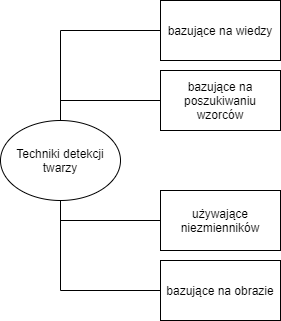
\includegraphics[width=7cm]{zdjęcia/techniki-detekcji.png}
	\caption{Techniki detekcji twarzy według Younga.} 
	\label{fig:detectionMethods}
\end{figure}

Charakteryzację każdej z grup \cite{Yang} można przedstawić w następujący sposób:
\begin{itemize}
    \item metody bazujące na wiedzy - wykorzustujące ludzkie obeznanie na temat elementów jakie zawiera przeciętna twarz
    \item techniki używające niezmienników - algorytmy skupiają się na zlokalizowaniu cech strukturalnych twarzy, które są niezmienne ze względu na kąt, oświetlenie, pozycję twarzy
    \item metody bazujące na przeszukiwaniu wzorcem - dzięki wielu zgromadzonym wzorcom odnośnie wyglądu twarzy lub jej konkretnych elementów poszukuje się korelacji między schematem a obrazem wejściowym
    \item metody bazujące na obrazie - model trenowany jest zestawem obrazów, które zawierają różnorodne ludzkie twarze, przedstawiane w zmiennych warunkach
\end{itemize}

Zagadnienie poruszane w tym rozdziale jest bardzo rozległe, a rozwiązania i algorytmy istniejące na rynku bardzo różnorodne. Większość powstałych implementacji łączy najlepsze cechy z kilku metod, przez co nie ma możliwości przypisania ich do konkretnej klasyfikacji. Ze względu na szeroki zakres tej 
tematyki oraz dużą ilość istniejących rozwiązań w dalszej części zostaną opisane dwa najpopularniejsze algorytmy, których implementacje są udostępniane przez biblioteki programistyczne.

% %---------------------------------------------------------------------------

\subsection{Schemat działania}
Dla omawianych poniżej algorytmów struktura programu wykrywania twarzy odbywa się dwuetapowo. Początkowym etapem jest wyszkolenie klasyfikatora, którego zadaniem będzie wykrycie twarzy. 

Następnie potrzebne jest działanie detektora skanującego cały obraz w celu lokalizacji istotnych cech takich jak oczy, usta, nos czy brwi. Ich rozpoznanie możliwe jest przez zgromadzone informacje znajdujące się w wytrenowanym wcześniej modelu.

Większość algorytmów uzależnia swoją efektywność od wielkości danych, na których został przeszkolony klasyfikator. Trenowanie na dużych zbiorach danych poprawia zdolność algorytmu w trakcie określenia czy na danym obrazie znajduje się twarz. \cite{fDetection}

% %---------------------------------------------------------------------------

\subsection{Klasyfikator kaskadowy z użyciem cech Haara}
\label{sub:Haar}
Paul Viola i Michael Jones w 2001 roku zaproponowali technikę wykrywania obiektów opartą o działanie klasyfikatora kaskad Haara (ang. Haar Feature-based Cascade Classifier) \cite{haar}. Pomimo wysokiej konkurencji ze strony sieci neuronowych, algorytm cieszy się ogromną popularnością po dzień dzisiejszy. Jego zastosowanie okazało się być przełomem w dziedzinie wykrywania twarzy. 

Działanie tej techniki łączy ze sobą poniższe koncepcje:
\begin{itemize}
    \item poszukiwanie i wybór najdokładniejszych cech Haara
    \item utworzenie zintegrowanych obrazów w celu szybkiego znalezienia danej cechy
    \item użycie metody sprawnego uczenia Adaboost
    \item zastosowanie klasyfikatora kaskadowego
\end{itemize}

Podejście to jest oparte o wytrenowanie klasyfikatora kaskadowego na wielu pozytywnych i negatywnych obrazach w skali szarości. Przez pierwszy rodzaj rozumie się zdjęcia zawierające twarze, natomiast jako próbki negatywne określa się zdjęcia, na których nie znajduje się twarz ludzka. Według zaleceń autorów algorytmu obrazy powinny mieć wymiary $24x24$ pikseli.

Pierwszym krokiem działania opisywanego modelu jest wydobycie ze wszystkich próbek odpowiednich cech Haara. Cechy te dotyczą zmian wartości kontrastu pomiędzy prostokątnymi grupami pikseli. W tym celu wykorzystuje się tak zwane funkcje Haara.

\begin{figure}[h]
	\centering
	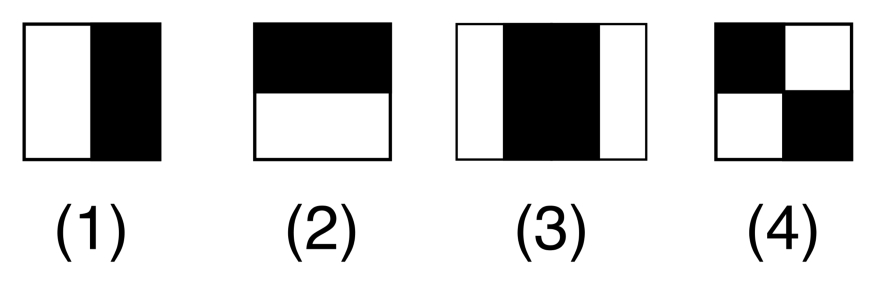
\includegraphics[width=6cm]{zdjęcia/haar_features.png}
	\caption{Przykładowe funkcje Haara. \cite{haarCascade}} 
	\label{fig:haarFeatures}
\end{figure}

Są to kombinacje prostokątów  o takich samych wymiarach (ciemnych i jasnych), pozwalające na detekcję konkretnych elementów. Funkcje dzielimy na trzy grupy, ze względu na ilość prostokątów (2, 3, 4) tworzących daną cechę. Na Rys. \ref{fig:haarFeatures} przedstawiono funkcje używane w tym algorytmie, wykorzystywane do wykrywania krawędzii na obrazie (1, 2) oraz prostych (3) i skośnych linii (4).

Każda funkcja Haara przemierza piksel po pikselu dany obraz. Dla każdego regionu (ciemnego jak i jasnego), który obejmuje owa cecha, sumowana jest wartość pikseli znajdujących się w tych obszarach. Następnie obliczana zostaje różnica między tymi sumami. Na podstawie tej różnicy, wyszukuje się lokalizację na obrazie, dla której dana cecha jest najbardziej odpowiednia. 

Przykładowo, na Rys. \ref{fig:haarNose} użyto funkcji złożonej z trzech prostokątów, o rozmiarze mającym na celu wykrycie oczu. Możliwe jest to poprzez fakt, iż obszar oczu jest ciemniejszy niż obszar nosa znajdujacy się pomiędzy nimi. Cechy Haara są pewnego rodzaju wzorcem, dla którego należy znaleźć najlepsze dopasowanie na obrazie.
 
\begin{figure}[h]
	\centering
	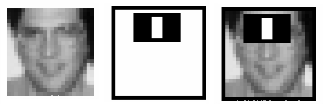
\includegraphics[width=5cm]{zdjęcia/haar_nose_feature.png}
	\caption{Zastosowanie funkcji Haara do wykrycia oczu i obszaru nosa.} 
	\label{fig:haarNose}
\end{figure}

Próba dopasowania cech Haara dla każdego piksela zawartego na obrazie, we wszystkich możliwych rozmiarach, wymaga wykonania niewyobrażalnej liczby działań. Rozwiązaniem jest stworzenie zintegrowanego obrazu, dzięki czemu złożoność obliczeń staje się dużo korzystniejsza.

Obrazem integralnym nazywamy reprezentację obrazu, w którym dana wartość $(x, y)$ równa jest sumie pikseli znajdujących się powyżej i na lewo od analizowanej lokalizacji (Rys. \ref{fig:integralImage}). Dana reprezentacja pozwala na przyspieszenie działań, jest to skuteczny sposób obliczenia sumy wartości pikseli dla prostokątnego podzbioru rozważanego obrazu.
 
 \begin{figure}[h]
	\centering
	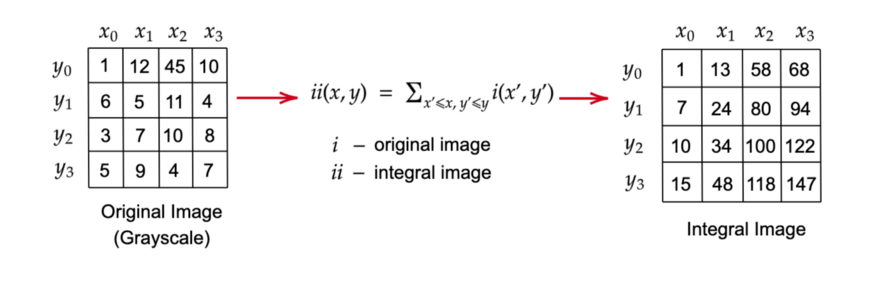
\includegraphics[width=14cm]{zdjęcia/integral.png}
	\caption{Konwersja na obraz zintegrowany. \cite{haarCascade}} 
	\label{fig:integralImage}
\end{figure}
 
Kolejnym krokiem jest wybór cech, które są istotne dla konkretnych obszarów. Ten efekt można osiągnąć z pomocą algorytmu Adaboost (ang. Adaptive Boosting). Jest to  algorytm uczenia maszynowego służący do wyboru najlepszych funkcji z całego ich zbioru. Owa technika wzmacniająca, poprzez zastosowanie wszystkich możliwych cech na każdym obrazie treningowym osobno, wybiera te o najniższym błędzie dla danej iteracji. Algorytm trenuje silny klasyfikator na podstawie liniowej kombinacji słabych klasyfikatorów.
 
Po wyborze najlepszych cech spośród wszystkich możliwości pozostaje etap zastosowania klasyfikatora kaskadowego. Z definicji, działa on wielostopniowo. Cechy wybrane jako kluczowe zostają podzielone na grupy, gdzie każda z nich odpowiada jednemu etapowi działania klasyfikatora. Pierwsze etapy zawierają niewiele funkcji, ale wybrane zostają te najbardziej pewne i charakterystyczne. 
 
Funkcje są nakładane na każde okno o zadanych wymiarach wyodrębniane na obrazie. W przypadku negatywnego rezultatu, tzn niedopasowania jednej z cech sprawdzanych w konkretnym etapie, analizowane okno jest od razu odrzucane. Nie rozważa się dla niego funkcji zawartych w dalszych etapach. Jeśli natomiast okno przejdzie pomyślnie wszystkie etapy działania klasyfikatora kaskadowego zostaje zaklasyfikowane jako obszar twarzy (Rys. \ref{fig:cascadeClasificator}).  
 
\begin{figure}[h]
	\centering
	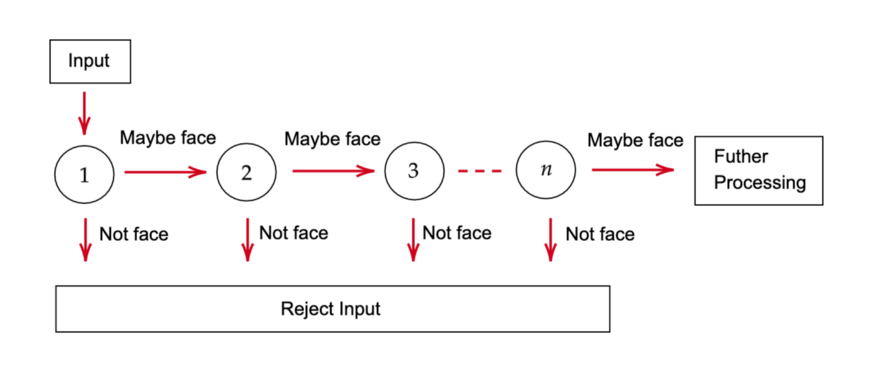
\includegraphics[width=14cm]{zdjęcia/haar_train.png}
	\caption{Klasyfikator kaskadowy. \cite{haarCascade}} 
	\label{fig:cascadeClasificator}
\end{figure}

W badaniu przeprowadzonym przez autorów algorytmu wybrano 6000 funkcji, które podzielono na 38 etapów klasyfikacji. Liczba cech w każdym z nich nie jest proporcjonalna, wynosi ona kolejno 1, 10, 25, 25, 50 funkcji dla pięciu pierwszych etapów. W początkowych etapach eliminujemy okna, w których nie ma elementówch charakterystycznych twarzy. Oszczędza to zbędnych obliczeń i analiz.

Opisany w tym rozdziale algorytm jest wykorzystywany nie tylko do wykrywania twarzy na obrazach, ale także innego rodzaju obiektów, takich jak zwierzęta, tablice rejestracyjne czy całe ludzkie sylwetki. Cechuje go bardzo szybki czas działania. Jego dokładność nie jest aż tak wysoka, ze względu na podatność na fałszywe wykrycia.  Popularność algorytmu, który został opisany w tym rozdziale, zdaje się dalej trwać, pomimo odkrycia wielu konkurencyjnych rozwiązań działających na podobnej zasadzie. 

% %---------------------------------------------------------------------------

\subsection{Klasyfikator SVM z użyciem deskryptora HOG}
\label{sec:svmhog}
W 2005 roku pojawiła się kolejna przełomowa propozycja metody wykrywania obiektów, w tym twarzy. Jej autorami są Navneet Dalal i Bill Triggs, którzy wykazali, że do trenowania modelu można skorzystać z deskryptora HOG (ang. Histograms of Oriented Gradients) oraz klasyfikatora SVM (ang. Support Vector Machine) \cite{hog}. 

Deskryptory wyodrębniają z obrazu przydatne informacje pomijając zbędne dane, pomagają zlokalizować konkretny, interesujący nas obiekt. W przypadku deskryptorów HOG  ekstrakcja cech odbywa się za pomocą histogramu gradientów, używanych jako cechy analizowanych obrazów. Jako gradienty określamy pola wektorowe wskazujące kierunek, w którym można obserwować znaczącą zmianę w intensywności koloru.

W celu stworzenia deskryptora HOG dla obrazu należy wykonać kilka istotnych kroków. \cite{hog2} Pierwszym z nich jest przygotowanie obrazu w odcieniach szarości, dla którego chcemy obliczyć histogram gradientów. Według autorów algorytmu rozmiar zdjęcia powinno się zmniejszyć do $128x64$ pikseli. Takie wymiary zostały wybrane ze względu na początkowe założenie wykrywania obiektów z tymże algorytmem. Miał on służyć do detekcji pieszych. Po sukcesie i dobrych wynikach, skupiono się na detekcji twarzy, w tym przypadku również zdecydowano się na wybór zdjęć o owych wymiarach.

Dla każdego piksela znajdującego się na obrazie należy obliczyć gradient pionowy i poziomy. Najprostszym sposobem jest filtracja obrazu przez poniższe jądra.

\begin{figure}[h]
	\centering
	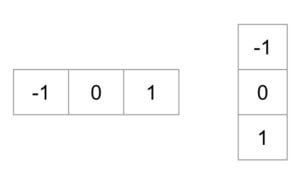
\includegraphics[width=5cm]{zdjęcia/hog-kernels.jpg}
	\caption{Jądra służące do filtracji obrazu w celu obliczenia gradientów. \cite{hog2}} 
	\label{fig:hogKernels}
\end{figure}

Aby znaleźć wielkość i kierunek każdego gradientu w danym bloku używa się określonych wzorów:
\begin{center}
    $g=\sqrt{g_{x}^{2}+g_{y}^{2}}$ ,
    $\theta=\arctan \frac{g_{y}}{g_{x}}$
\end{center}

Kolejnym krokiem jest podział obrazu na jednakowe siatki o wymiarach $8x8$. Każdą komórkę da się przedstawić za pomocą 128 liczb. Pojedynczy fragment składa się z 64 pikseli, z każdym związane są ważne wartości dotyczące jego gradientu - wielkość i kierunek ($8x8x2 = 128$). 

Aby skompresować dane dla każdej siatki, należy stworzyć histogram z podziałem na dziewięć oddzielnych pojemników. Każdy z nich odpowiada kątom z zakresu 0-160 z 20-stopniowym przyrostem.

Przyporządkowując każdy piksel do jednego z pojemników uwzględnia się kierunek gradientu (jego kąt) oraz wielkość, która go charakteryzuje. Pojemnik jest wybierany ze względu na kąt, natomiast wpisywana do niego wartość to wielkość przypisana do danego gradientu. Jeżeli piksel leży w połowie odległości między dwoma pojemnikami, jego wartość dzieli się miedzy oba pola. Omawiana sytuacja dotyczy piksela oznaczonego na czerwono na Rys. \ref{fig:gradientHistogram}. 

Ważną kwestią jest rozważenie przypadku, gdy analizowany kąt posiada miarę większą niż 160 stopni (maksymalna wartość kąta w pojemniku). W takim przypadku wartość gradientu takiego piksela jest dzielona proporcjonalnie między dwa pojemniki, pierwszy i ostatni.

\begin{figure}[h]
	\centering
	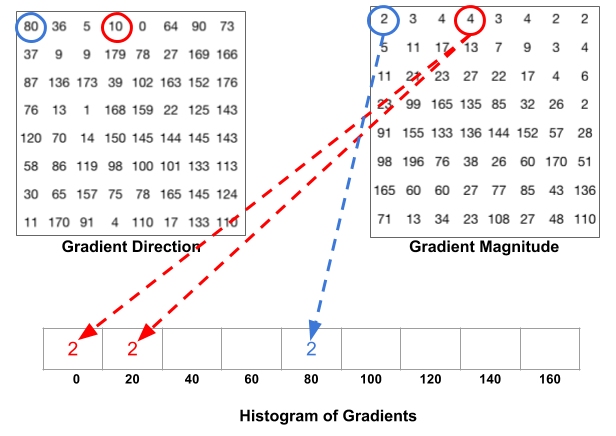
\includegraphics[width=10cm]{zdjęcia/gradients-histogram.png}
	\caption{Schemat tworzenia histogramu dla komórki o wymiarach $8x8$. \cite{hog2}} 
	\label{fig:gradientHistogram}
\end{figure}

Po wykonaniu procesu dla wszystkich pikseli można zobaczyć w jaki sposób rozkładają się wartości w zależności od kierunku gradientu charakteryzującego każdy z nich. Taka reprezentacja zapewnia odporność na szum, który istnieje między gradientami na samym początku. 

Gradienty obrazu są wrażliwe na oświetlenie. W przypadku zmiany jego natężenia, wielkość gradientów diametralnie się zmienia. Aby uodpornić deskryptor na jego wpływ stosuję się normalizację histogramu. 

Bloki przekształca się w wektory elementów, a następnie dla każdego stosuje się normalizację. Blok o wymiarach $16x16$ posiada 4 histogramy, gdzie każdy da się przedstawić jako wektor $9x1$ co w sumie daje wektor $36x1$. Normalizacja następuje dla pierwszego okna, po czym jest ono przesuwane o 8 pikseli gdzie znormalizowany wektor jest obliczany ponownie. Wszystko powtarza się do momentu przebycia wszystkich pozycji.

Każdy z omawianych bloków reprezentowany jest przez wektor $36x1$ co jest równoznaczne z 36 wyodrębnionymi cechami. Istnieje 105 pozycji takich bloków (7 poziomych, 15 pionowych). Sumarycznie dla naszego zdjęcia otrzymujemy aż 3780 cech.

Powyżej zostało opisane działanie deskryptora HOG na pojedynczym obrazie. Jest on podstawą rozpatrywanego algorytmu, którego celem jest stworzenie programu wykrywającego twarze. Aby osiągnąć takową użyteczność, należy połączyć działanie deskryptora z klasyfikatorem SVM.

Klasyfikator SVM pozwala na analizę danych, rozpoznanie wzorców i ich klasyfikację. Do jego wytrenowania używa się próbek pozytywnych i negatywnych, tak jak w przypadku przygotowywania klasyfikatora kaskadowego.

Z każdego zdjęcia, za pomocą deskryptora, należy wyciągnąć cechy HOG. Na ich podstawie trenuje się klasyfikator SVM. Uczy on się różnych możliwych cech twarzy, które potem próbuje zlokalizować na nowym zdjęciu. Po fazie uczenia, klasyfikator pozwala określić do jakiej klasy należą przetwarzane dane. W naszym przypadku rozróżni on fragment zawierający twarz i ten na którym się ona nie znajduje. 

Analizowana w tej sekcji metoda stała się konkurecją dla algorytmu opisywanego we wcześniejszym podrozdziale. Dokładność jego działania jest dużo lepsza niż algorytmu opartego na klasyfikatorze kaskadowym. Minusem jest wykrywanie twarzy tylko w przypadku widoku z przodu, program nie działa poprawnie w momencie jej rotacji i zmian kąta.

Podobnie jak poprzedniczka, pomimo wielu innych propozycji algorytmów, które pojawiły się od roku 2005, ten algorytm wciąż cieszy się wielką popularnością. Zdaje się być prosty i efektywny, pomimo wolniejszego działania.

% %---------------------------------------------------------------------------

\section{Identyfikacja punktów charakterystycznych}
\label{sec:landmarks}
Opisana wcześniej technika wykrywania twarzy jest początkowym etapem algorytmu, który zostanie przedstawiony w niniejszej sekcji. Mowa tutaj o algorytmie detekcji punktów charakterystycznych twarzy (ang. facial landmarks), poprzez których pojęcie rozumie się elementy, pomagające zidentyfikować jej najistotniejsze cechy. Zazwyczaj są to punkty utożsamiane z linią szczęki, ust, nosa, oczu i brwi. \cite{landmarks2}

Schemat wykrywania owych elementów działa dwuetapowo. Pierwszym krokiem jest lokalizacja twarzy. Metoda, która zostanie do tego wykorzystana nie jest istotna. Ważne jest uzyskanie ograniczonego obszaru, aby następnie można było rozpocząć wykrywanie kluczowych struktur. 

Tak jak w innych przypadkach, istnieje wiele różnych propozycji rozwiązania tego problemu. Algorytm, który aktualnie cieszy się dużą popularnością został zaproponowany w 2014 roku, a jego działanie opiera się na wykorzystaniu drzew regresji. Jego autorami są Vahid Kazemi oraz Josephine Sullivan. 

\begin{figure}[h]
	\centering
	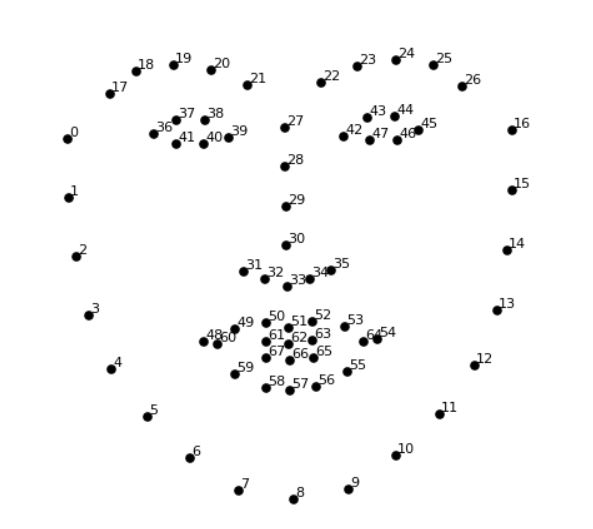
\includegraphics[width=8cm]{zdjęcia/landmarks_points.JPG}
	\caption{Wizualizacja 68 punktów charakterystycznych twarzy.} 
	\label{fig:landmarks}
\end{figure}

Działanie tej techniki \cite{landmarks} można opisać w następujący sposób:
\begin{itemize}
    \item Jako zbiór testowy wybiera się taki zestaw danych, który składa się z obrazów z oznaczonymi ręcznie punktami charakterystycznymi twarzy.
    \item Następnie model zostaje szkolony za pomocą drzew regresji na podstawie samej intensywności pikseli i próby dopasowania punktów w odpowiednie miejsca.
    \item  Korzysta się z obliczania prawdopodobieństwa odległości między parami pikseli.
    \item Celem treningu jest optymalizacja funkcji błędu i dokonanie selekcji odpowiednich cech w oparciu o dane zawarte w zbiorach.
\end{itemize}

Rezultatem powyższych działań jest model zdolny do zlokalizowania charakterystycznych obszarów twarzy. W artykule, w którym pierwszy raz zaproponowano to rozwiązanie, testowano algorytm na zbiorze danych umożliwiającym wykrycie aż 192 istotnych punktów. Popularne biblioteki, w tym dlib, często udostępniają wariant wytrenowany na innym zbiorze danych. Zazwyczaj są to obrazy, na których oznaczono 68 kluczowych pozycji punktów (Rys. \ref{fig:landmarks}).

Zaletą przedstawionego algorytmu jest niezwykle szybki czas działania oraz dobra dokładność wykrywania elementów, nawet w przypadku twarzy ukazanych z profilu. Plusem jest także możliwość użycia dowolonych danych treningowych, czego efektem jest wyszkolenie własnego detektora punktów nie tylko twarzy, ale też własnych niestandardowych elementów.

Technika, która została omówiona w tym rozdziale znajduje swoje zastosowania w wielu dziedzinach życia. Często jest ona uzupełnieniem wykrywania twarzy, w celu upewnienia się co do tożsamości danych osób. Jest to przydatny system w analizowaniu emocji ludzi, pozwala osobom z autyzmem bądź innymi chorobami lepiej zrozumieć otaczający ich świat. W przypadku oprogramowania czytającego z ruchu warg również analizuje się zmiany lokalizacji ważnych punktów charakterystycznych.

% %---------------------------------------------------------------------------

\section{Triangulacja Delaunaya}
Poprzez pojęcie triangulacji, w kontekście matematycznym, można rozumieć podział figury geometrycznej na trójkąty, bądź też czworościany (określane jako sympleksy) w taki sposób, aby część wspólna dwóch sąsiadujących trójkątów (czworościanów) była ich wspólną ścianą, wierzchołkiem, bokiem, trójkątem lub zbiorem pustym. \cite{triangulation}

Istnieje wiele różnych rodzajów triangulacji. W przypadku rozważanego w tej pracy algorytmu wykorzystano triangulacje zbioru punktów, do której należy między innymi triangulacja Delaunaya (lub Delone), której nazwa pochodzi od nazwiska autora tejże koncepcji Borysa Delaunaya. 

Triangulacja Delone \cite{tDelone} rozumiana jest jako triangulacja $T$ przestrzeni $R^{n+1}$, którą definiuję się w poniższy sposób. Jako $T$ określa się podział przestrzeni $R^{n+1}$ na $(n+1)$ sympleksów, z punktami jako wierzchołki, spełniających okreśone warunki:

\begin{enumerate}
    \item każde dwa sympleksy należące do zbioru $T$ posiadają wspólną ściane albo nie są ze sobą połączone w żaden sposób
    \item każdy z ograniczonych zbiorów w przestrzeni $R^{n+1}$ ma część wspólną z ograniczoną liczbą trójkątów ze zbioru $T$
    \item opisując kulę na dowolonym trójkącie ze zbioru $T$ nie natkniemy się na sytuację, gdy wnętrze kuli będzie zawierało wierzchołki z pozostałych sympleksów zawartych w zbiorze $T$
\end{enumerate}

\begin{figure}[h]
	\centering
	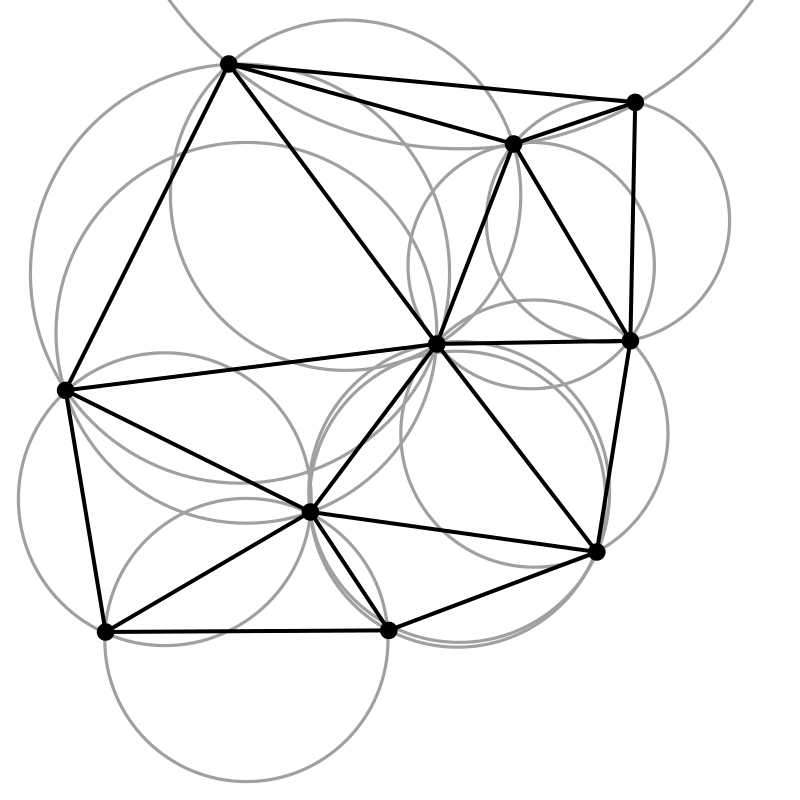
\includegraphics[width=6cm]{zdjęcia/triangulation.png}
	\caption{Przykładowa triangulacja Delone dla zbioru punktów. \cite{tDelone}}
	\label{fig:delone}
\end{figure}

Wspominając o triangulacji Delone warto wspomnieć o diagramach Voronoi, które są ściśle powiązane z owym pojęciem. Diagram Voloroi dla zestawu punktów dzieli przestrzeń w taki sposób, że linie podziału znajdują się w równej odległości od punktów sąsiadujących.

Ważną własnością trangulacji Delone jest fakt, iż wraz z diagramem Voronoi tworzy ona graf dualny. Te definicje są powiązane, więc znając trangulację Delone dla zbioru punktów możemy w łatwy sposób obliczyć diagram Voronoi. Dwa trójkąty mające wspólną krawędź w triangulacji umożliwiają odnalezienie krawędzie w diagramie Voronoi. 

Centra okręgów wyznaczonych przez owe trójkąty po połączeniu tworzą daną krawędź. Rys. \ref{fig:voronoi}  przedstawia krawędzie triangulacji (czarne linie) oraz utworzone na podstawie triangulacji komórki Voronoi (czerwone linie).

\begin{figure}[h]
	\centering
	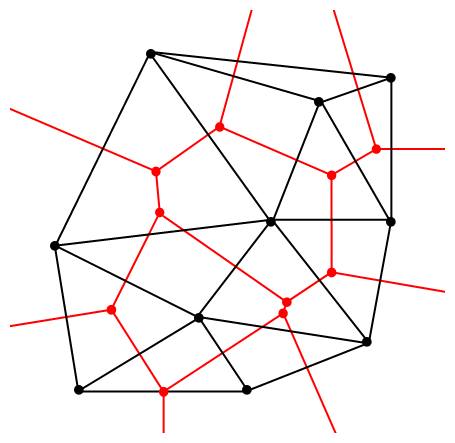
\includegraphics[width=6cm]{zdjęcia/voronoi.png}
	\caption{Graf przedstawiający komórki Vornoi oraz krawędzie triangulacji. \cite{tDelone}} 
	\label{fig:voronoi}
\end{figure}

Istotną własnością tej techniki jest fakt, że trójkąty powstałe w wyniku triangulacji nie mają kątów o dużych miarach, co zapewnia przejrzystość wygenerowanych figur. W przypadku zastosowania triangulacji na zbiorze punktów można uniknąć chaosu i nierównomierności.

Triangulacja ma swoje zastosowania w wielu dziedzinach. Wykorzystuje się ją w informatyce, grafice komputerowej czy też geodezji. Technika umożliwia tworzenie skomplikowanych figur, wypełnianie obszarów, wyznaczanie linii przecięcia.

Istnieje wiele różnych algorytmów przeznaczonych do znajdowania trangulacji Delone dla zbioru punktów. Przedstawienie ich w niniejszej pracy dyplomowej nie jest jednak kluczowe. Większość języków programowania dostarcza odpowiednie biblioteki, które posiadają funkcje implementujące takowe algorytmy. 


% Istnieje wiele różnych algorytmów przeznaczonych do znajdowania trangulacji Delone dla zbioru punktów. Nie jest to jednak kluczowe w przypadku niniejszej pracy dymplomowej. W implementacji zostanie użyta odpowiednia biblioteka, która implementuje algorytm triangulacji Delone. 

% W przypadku tworzenia algorytmu animacji awatara istotne jest, aby trójkąty tworzone ze zbioru punktów charakterystycznych były zbudowane w odpowiedni sposób. Trójkąty powstałe w wyniku triangulacji nie będą mieć dużych kątów, co zapewni przejrzystość powstałych figur. W przypadku podziału twarzy na takowe figury unikniemy chaosu, nierównomierności. Właśnie dlatego zdecydowałam się na wybór tejże techniki.



\chapter{Przegląd istniejących zastosowań}

Niemal każdy z nas na co dzień używa smartfona i korzysta z różnego rodzaju aplikacji, których celem jest komunikacja z ludźmi, zarządzanie finansami, tworzenie notatek, dokumentów bądź też zapewnienie rozrywki użytkownikowi. W czasach, w których media społecznośiowe odgrywają znaczącą rolę popularne stało się stosowanie filtrów modyfikujących twarz, sylwetkę lub dodających do zdjęć efekty specjalne. 

Zgłebiając zasoby internetowe łatwo natrafić na narzędzia, które stosują rozwiązania zbliżone do implementowanego w niniejszej pracy algorytmu.

W tym rozdziale zostanie opisana technika deepfake, która z dnia na dzień zyskuje na popularności. Zostaną również przedstawione przykładowe aplikacje mobilne implementujące ową technikę i oparte o wykorzystanie sztucznej inteligencji w przetwarzaniu obrazów. 

% %---------------------------------------------------------------------------

\section{Technika deepfake}
Technologia deepfake umożliwia przedstawienie dowolnej osoby jako uczestnika danego filmu, czy też postaci znajdującej się na konkretnym zdjęciu. Jej celem jest zamiana wypowiedzi jednej osoby, na wypowiedź innej, to samo dotyczy ruchów ciała. Istnieje także możliwość spreparowania dźwięku, przez co mamy wrażenie, że słyszymy słowa wypowiadane przez znajomą nam osobę, tymczasem jest to fikcja uzyskana z pomocą sztucznej inteligencji. Owa technika to symulacja rzeczywistości, często wykorzystywana we współczesnym kinie w przypadku generowania komputerowych scenografii.

Kiedy podczas kręcenia siódmej części filmu Szybcy i Wściekli zmarł Paul Walker kierownicy produkcji musieli zmierzyć się z niemałym na tamte czasy wyzwaniem, symulując sceny z jego udziałem. W dzisiejszych czasach technologia deepfake niezwykle się rozwinęła i stała się bardzo popularna, każda osoba ma możliwość wygenerowania filmu będącego deepfake'iem w kilka minut.

Słowo deepfake to tak naprawdę połączenie dwóch angielskich wyrazów. Nawiązuje ono do technologii uczenia głębokiego (ang. deep learning), z którą owa technika jest ściśle związana, oraz do słowa fake oznaczającego coś nieprawdziwego, udającego inną rzecz.

Działanie algorytmu deepfake często oparte jest na wykorzystaniu autoenkoderów lub sieci GAN (ang. Generative Adversarial Network). Według wielu osób wspomniane wyżej sieci mogą być związane z ogromnym rozwojem tejże technologii. Podobizny, które zostają wygenerowane poprzez ich zastosowanie wydają się być prawie nieodróżnialne od rzeczywistych twarzy \cite{deepfake}.

Stworzenie filmu określanego jako deepfake musi zostać poprzedzone przez odpowiednie procedury. Na przykładzie enkoderów pierwszym krokiem jest przepuszczenie zdjęcia źródłowego jak i docelowego przez enkoder, który uczy się podobieństw między dwoma twarzami. Następnie dane są kompresowane, wyciągane są wspólne cechy obydwu zdjęć. Kolejnym etapem jest wytrenowanie dwóch dekoderów, które zostaną użyte to odzyskania twarzy każdej z osób. Ostatnim krokiem jest podmiana twarzy między dekoderami. Dekoder ma za zadanie zrekonstruować twarz drugiej osoby na podstawie orientacji pierwszego obrazu. 

Sieci GAN działają inaczej, na początku zostają trenowane poprzez kilkugodzinne analizowanie rzeczywistego filmu wideo. Dzięki temu są w stanie nauczyć się jak wygląda twarz osoby pod różnymi kątami, w różnym świetle. Następnie łączy się wytrenowaną sieć z technikami grafiki komputerowej, nakłada się kopię osoby na danego aktora. Wszystko odbywa się poprzez mapowanie odpowiednich punktów charakterystycznych twarzy.

Technologia deepfake niesie ze sobą niemałe zagrożenie. Poziom zaawansowania sprawia, że czasami ciężko na pierwszy rzut oka wykryć film, na którym została zastosowana. Na dzień dzisiejszy dzięki dokładniejszej analizie takowego wideo jesteśmy w stanie wykryć czy stworzony film jest fikcją. Jednak według wielu przypuszczeń, niewykluczone, że wraz z rozwojem sztucznej inteligencji przestanie to być możliwe.

% %---------------------------------------------------------------------------

\section{Dostępne aplikacje mobilne}

\subsection{Wombo.ai}
Wombo.ai \cite{womboai} to bardzo popularna, darmowa aplikacja mobilna, która została stworzona w celu rozrywkowym. Jest ona dostępna zarówno na smartfony jak i tablety z systemem operacyjnym Android i IOS, co zdecydowanie jest jej walorem. Reprezentowaną przez nią ideą jest tworzenie zabawnych filmików, na których ożywiane są wgrane wcześniej fotografie. Zaletą tej aplikacji jest jej prostota i łatwość w obsłudze. 

Wszystko odbywa się w kilku krokach, należy zrobić zdjęcie swojej twarzy albo wgrać takowe z galerii, następnie wybrać utwór muzyczny na podstawie którego otrzymujemy krótkie nagranie ze stworzoną animacją. Filmiki zostają wygenerowane z użyciem technologii deepfake przez co są bardzo realistyczne. Jej działanie powiązane jest z wykorzystaniem sztucznej inteligencji do synchronizowania ruchu.

% %---------------------------------------------------------------------------

\subsection{Anyface: face animation}
Anyface \cite{anyface} to aplikacja mająca na celu, podobnie jak poprzedniczka, zapewnienie rozrywki użytkownikowi. Jest ona dostępna w wersji mobilnej tylko na Androida.

W odróżnieniu do wspomnianego wyżej programu to narzędzie posiada dużo więcej funkcji, przez co może sprawiać wrażenie bardziej atrakcyjnego dla użytkownika. Poza animacją zdjęcia na podstawie wybranej frazy istnieje możliwość dodania własnego nagrania, z którego użyciem zostanie wygenerowana animacja. Narzędzie posiada także moduł edycji i udoskonalania zdjęć, odbiorca jest w stanie dodawać filtry, efekty specjalne i inne obiekty, które nadadzą animacji unikalny charakter. 

% %---------------------------------------------------------------------------

\subsection{MotionPortrait}
MotionPortrait \cite{motionportrait} to bardzo podstawowa aplikacja mobilna dostępna zarówno na Androida jak i system IOS. Kategoria, w której można ją znaleźć to rozrywka. Posiada opcję zrobienia własnego zdjęcia, dodania zdjęcia z galerii lub wyboru udostępnionej fotografii. Po wykonaniu tego etapu mamy możliwość animacji naszej podobizny poprzez wybór zdefiniowanych wyrazów twarzy. 

Dzięki połączeniu z mikrofonem w przypadku wypowiadania jakichkolwiek słów nasza twarz jest animowana. Animacja dotyczy tutaj tylko ust, awatar mruga regularnie oczami. Efekt, który otrzymujemy nie jest zbyt satysfakcjonujący. Na zdjęcie możemy też nałożyć różne filtry, dodać efekty. Ostatecznie istnieje możliwość nagrania krótkiego wideo, które potem możemy zapisać.

% %---------------------------------------------------------------------------

\section{Wnioski}
Na rynku dostępna jest duża ilość aplikacji podobnych do programów opisanych powyżej. Niektóre z nich są bardzo podstawowe a efekty osiągane przez te narzędzia nie wydają się być spektakularne. Istnieją jednak rozwiązania, które odstają od innych swoją dokładnością działania i efektowną realizacją. 

Pewne jest, że użytkownicy chętnie korzystają z owych aplikacji. Przeglądając media społecznościowe na każdym kroku możemy się natknąć na filmiki stworzone z użyciem techniki deepfake. Co więcej, narzędzia oparte na tych technologiach niezwykle szybko się rozwijają i zaczynają zaskakiwać swoimi opcjami.

Powyższe fakty sprawiają, że stworzenie algorytmu animacji awatara w ramach tejże pracy inżynierskiej wydaje się być sensowne. Są to narzędzia, które wykorzystuje się nie tylko w celu rozrywkowym, ale także w dziedzinie kinematografii. 



\chapter{Wykorzystane narzędzia i technologie}
\label{cha:wykorzystaneNarzedziaITechnologie}
W niniejszym rozdziale zostaną zawarte krótkie opisy narzędzi oraz technologii wykorzystanych w trakcie implementacji algorytmu będącego tematem owej pracy inżynierskiej. Zostanie również przedstawiony język programowania, w którym stworzono projekt, oraz charakteryzujące go zalety przeważające o jego wyborze. 

% %---------------------------------------------------------------------------

\section{Python}
Język programowania Python \cite{PythonWiki} powstał we wczesnych latach dziewięćdziesiątych. Guido van Rossum jest uważany za głównego twórcę tego języka, jednak wkład w jego rozwój miały także inne osoby. 

Popularność narzędzia wzrosła diametralnie w momencie wydania wersji $2.0$ w roku 2000 i rośnie aż do teraz. Aktualnie znajduje się on w czołówce najczęściej wykorzystywanych języków (Rys. \ref{fig:programmingLang}). Jego interpretery dostępne są na wiele systemów operacyjnych, obsługuje większość używanych w dzisiejszych czasach platform, takich jak Windows, Linux, AIX, iOS i inne.

\begin{figure}[h]
	\centering
	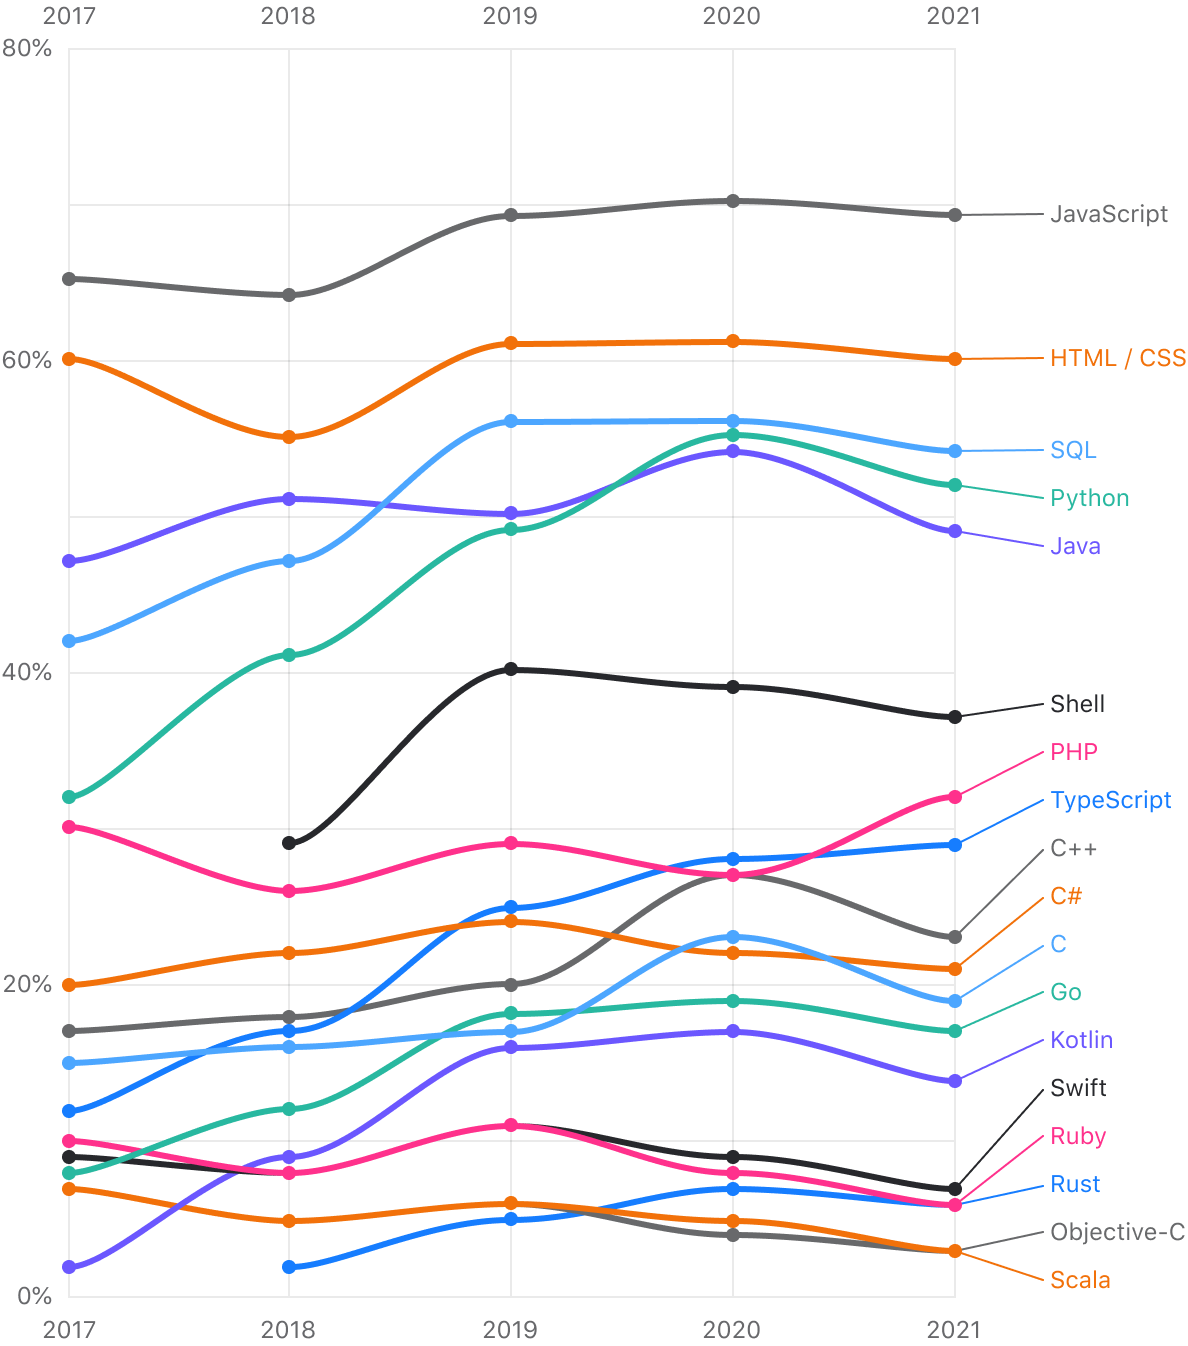
\includegraphics[width=7cm]{zdjęcia/python.png}
	\caption{Popularność wybranych języków programowania na przestrzeni lat} 
	\label{fig:programmingLang}
\end{figure}

Projekt, w ramach którego zostaje rozwijany owy język zarządzany jest przez Python Software Foundation, będącą organizacją non-profit. Narzędzie zostało udostępnione jako otwarte oprogramowanie, przez co użytkownicy posiadają możliwość ingerowania w wydawany kod źrodłowy.

Python to język wielopoziomowy, którego przeznaczenie nie jest ściśle określone. Jego możliwości są niezwykle rozległe i uzależnione od stosowanych bibliotek, platform oraz gotowych skryptów, których wybór jest wyjątkowo obszerny. 

Język nie wymusza od użytkownika jednego stylu, w którym tworzone są programy. Istnieje możliwość zastosowania różnych paradygmatów programowania (obiektowe, strukturalne oraz funkcyjne), co zdecydowanie wpływa na rozległość jego zastosowań. Ważną kwestią jest także dynamiczność, którą oferuje. Podczas tworzenia zmiennych nie wymaga się definiowania ich typu. Co więcej Python posiada automatyczne zarządzanie pamięcią, które zwalnia programistę z tego obowiązku. 

Główną ideą towarzyszącą twórcy podczas opracowywania składni języka była wysoka czytelność kodu źródłowego, jego przejrzystość i zwięzłość. Okazało się to jednym z głównych czynników, które spowodowały, że stał się tak powszechnie wykorzystywany.

Dzięki swojej uniwersalności Python odnajduje zastosowanie w wielu różnych dziedzinach, które zostały przedstawione na Rys. \ref{fig:pythonUsage}. 

\begin{figure}[h]
	\centering
	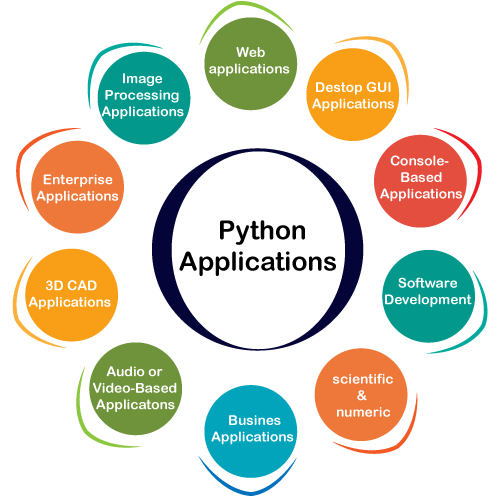
\includegraphics[width=7cm]{zdjęcia/python_usage.png}
	\caption{Dziedziny, w których najczęściej wykorzystuje się język programowania Python} 
	\label{fig:pythonUsage}
\end{figure}

Popularność w środowisku matematycznym zawdzięcza bibliotece SciPy stanowiącą darmową alternatywę do języka Matlab. 

Biblioteka Tensor Flow wspiera tworzenie sieci neuronowych, wykorzystywane w tworzeniu algorytmów w popularnych aplikacjach \cite{PythonApps}. W przypadku dziedzin operujących na przetwarzaniu obrazów czy też analizowaniu danych Python dostarcza kilka pakietów ułatwiających te operacje.

Ze względu na powyższe fakty, to jest między innymi czytelność, uniwersalność oraz ogromne zasoby pakietów, algorytm będący tematem niniejszej pracy inżynierskiej został opracowany w języku Python. W następnej sekcji zostaną przedstawione biblioteki wykorzystane w jego implementacji.

% %---------------------------------------------------------------------------

\section{Biblioteki}
Biblioteki programistyczne dostarczają podprogramy, które użytkownik może wykorzystać w swoim kodzie źródłowym bez konieczności implementowania ich od podstaw. Jest to metoda na wielokrotne używanie identycznego kodu.

% %---------------------------------------------------------------------------

\subsection{OpenCV}
Biblioteka OpenCV \cite{opencv} jest narzędziem wydanym jako otwarte oprogramowanie, wspomagające przetwarzanie obrazów oraz uczenie maszynowe. Została napisana w języku C, natomiasto posiada interfejsy dla innych języków, takich jak Java, Python bądź Matlab.

Zawiera około 2500 zoptymalizowanych algorytmów implementujących między innymi wykrywanie i rozpoznawanie twarzy, identyfikację i śledzenie ruchu obiektów. Znajdują się w niej także moduły dotyczące modeli 3D, ich tworzenia i przetwarzania.

Poza skomplikowanymi algorytmami OpenCV dostarcza wiele podstawowych operacji, które wykorzystuje się przy modyfikacji obrazów. Zaimplementowane funkcje zdają się wyróżniać wydajnością, co jest bardzo istotne w przypadku działania na dużych zbiorach danych.

% %---------------------------------------------------------------------------

\subsection{imutils}
Pakiet imutils \cite{imutils} to kolejne przydatne narzędzie wykorzystywane w trakcie modyfikacji obrazów. Zawiera szereg funkcji ułatwiających ich przetwarzanie, takich jak obracanie, zmiana rozmiaru, przesunięcie, zastosowanie szkieletyzacji. Zaimplementowano także moduły ułatwiające poprawną prezentację zdjeć podczas ich wyświetlania.

Funkcje zawarte w owym pakiecie pochodzą z biblioteki OpenCV, zostały one odpowiednio połączone i zmodyfikowane, aby można było w prostszy sposób dokonywać podstawowych operacji na zdjęciach. Biblioteka OpenCV zawiera ogromną ilość komponentów, co może być przytłaczające dla osoby rozpoczynającej swoją przygodę z przetwarzaniem obrazów.

Ideą, dla której powstał tenże pakiet była chęć zebrania podstawowych modułów i odpowiednie ich dostosowanie w celu ograniczenia zbędnych operacji, które należy zastosować korzystając z biblioteki OpenCV.

% %---------------------------------------------------------------------------

\subsection{dlib}
Dlib to biblioteka udostępniona na zasadach otwartej licencji, napisana w języku C++ \cite{dlib}. Dostarcza ona algorytmy oparte o uczenie maszynowe oraz narzędzia do tworzenia oprogramowania we wspomnianym wyżej języku. 

Funkcje, z których można korzystać, implementują algorytmy umożliwiające wytrenowanie klasyfikatorów SVM, SVR czy też klasyfikatory bez nadzoru. Dodatkowo istnieje możliwość wytrenowania własnego modelu wykrywającego twarz lub jej punkty charakterystyczne.

Zastosowania tej biblioteki obejmują takie dziedziny jak przemysł, robotyka oraz wszelkie obszary wymagające skorzystania z programów o dobrej wydajności obliczeniowej.

% %---------------------------------------------------------------------------

\subsection{scikit-image}
Biblioteka scikit-image \cite{skimage}, podobnie jak opisane powyżej pakiety, zawiera szereg implementacji algorytmów powiązanych z przetwarzaniem obrazów. Została udostępniona jako otwarte oprogramowanie tworzone przez kilkadziesiąt osób. 

Obejmuje ona takie algorytmy jak transformacje, segmentacje obrazów, ich morfologię oraz manipulację przestrzenią kolorów. Pakiet korzysta z tablic biblioteki NumPy, wykorzystanych do przechowywania obrazów.

% %---------------------------------------------------------------------------

\section{Flask}
Flask \cite{flask} to minimalistyczny szkielet wspierający tworzenie aplikacji webowych (ang. microframework). Zawiera wiele przydatnych bibliotek oraz modułów umożliwiających ich proste implementowanie.

W odróżnieniu od pełnowymiarowej platformy programistycznej (ang. framework) nie posiada warstwy abstrakcji bazy danych, części walidacyjnej formularzy czy też innych elementów, które wymagałaby zapewnienia szczególnych bibliotek. Natomiast obsługuje rozszerzenia, ktore umożliwiają dodanie owych funkcji do aplikacji.

Flask dostarcza programiście wiele przydatnych modułów, dzięki którym nie musi się on zajmować obsługą wątków i protokołów. Oparty jest na zestawie kilku narzędzi, na które składają się:
\begin{itemize}
\item Werkzeug - biblioteka udostępniająca zestaw narzędzi WSGI (ang. Web Server Gateway Interface) rozumianych jako interfejs bramy serwera WWW. Implementuje on przetwarzanie żądań między serwerem a aplikacją
\item jinja2 - biblioteka programistyczna umożliwiająca osadzanie danych na stronie w odpowiednich szablonach prezentacyjnych, której rezultat jest widoczny w przeglądarce
\item MarkupSafe - biblioteka rozszerzająca typ tekstowy, zapewniająca bezpieczne używanie znaków w HTML oraz XML. Zabezpieczna przed atakami poprzez wprowadzanie niezauwanych danych
\item ItsDangerous - pakiet odpowiadający za poprawną serializację danych. Służy do przechowywania sesji za pomocą plików cookies
\end{itemize}

Głównymi zaletami opisywanego szkieletu jest jego prostota i brak ograniczeń związanych ze ściśle ustalonymi regułami, którymi należy się kierować budując program. Jest niezwykle elastyczny, nadaje się do tworzenia małych, wewnętrznych aplikacji, ale jednocześnie daje możliwość rozbudowania ich do pełnowymiarowej struktury. 

W związku z wymienionymi zaletami, Flask zdaje się być idealnym narzędziem do stworzenia prostej aplikacji mającej na celu walidację algorytmu tworzonego w owym projekcie.

% %---------------------------------------------------------------------------

\section{Pycharm}
Pycharm \cite{pycharm} jest zintegrowanym środowiskiem wspierającym dla języka programowania Python. Oprogramowanie jest dostępne na wielu platformach systemowych takich jak Windows, Linux i macOS. Oferuje inteligentny edytor kodu źródłowego z możliwością formatowania i autouzupełniania, który posiada funkcję weryfikacji błędów oraz ich kontrolowanie.

Zapewnia refaktoryzację języka, przez co utrzymana jest wysoka jakość systemowa. Elementy są wpasowywane w dane wzorce, dopasowywane do obowiązujących standardów.

Ważną kwestią jest udostępniane wsparcie dla różnych bibliotek i narzędzi. Pycharm wspiera tworzenie stron internetowych z wykorzystaniem biblioteki Django, czy też Flaska i Pyramid. Wspomaga tworzenie plików w językach powiązanych z technologią webową (HTML, CSS, JavaScript).

Ułatwia pracę z projektem dostarczając prosty interfejs konfiguracyjny. W przypadku tworzenia aplikacji webowej opartej na platformie Flask w nieskomplikowany sposób można wprowadzić wszystkie istotne ustawienia.







\chapter{Algorytm animacji awatara}
\label{cha:implementacja}
Jak wspomniano we wcześniejszych rozdziałach, działanie algorytmu zaimplementowanego na potrzeby tej pracy inżynierskiej można podzielić na kilka kluczowych etapów. Poniższy rozdział zawiera szczegółowy opis każdego z nich. Zostaną także zaprezentowane efekty otrzymane w konkretnych krokach.

\section{Struktura programu}
Do stworzenia algorytmu wykorzystano język programowania Python umożliwiający tworzenie różnego rodzaju funkcji. Zostały one zaimplementowane dla każdego istotnego etapu programu, które zostały przedstawione na poniższym schemacie (Rys. \ref{fig:algorithmStructure}).

\begin{figure}[h]
	\centering
	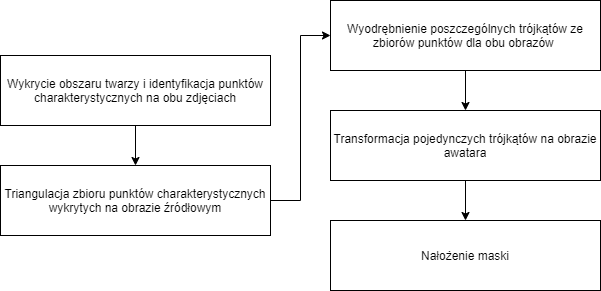
\includegraphics[width=14cm]{zdjęcia/struktura.png}
	\caption{Etapy algorytmu animacji awatara.} 
	\label{fig:algorithmStructure}
\end{figure}

Kluczową kwestią jest wcześniejsze wczytanie danych, czyli obrazu źródłowego, przez który rozumie się zdjęcie mające posłużć jako baza do przekształcenia awatara oraz jego obraz, na którym nastąpi animacja.

% \begin{itemize}
%     \item Wykrycie obszaru twarzy i identyfikacja punktów charakterystycznych na obydwu zdjęciach
%     \item Triangulacja zbioru punktów charakterystycznych wykrytych na obrazie źródłowym
%     \item Wyodrębnienie odpowiadających sobie sympleksów ze zbiorów punktów 
%     \item Transformacja pojedynczych trójkątów
%     \item Nałożenie maski 
% \end{itemize}

\section{Wykrycie twarzy oraz punktów charakterystynczych}
Pierwszym krokiem jest wykrycie obszaru twarzy oraz identyfikacja jej punktów charakterystycznych. Zostało to zrealizowane z użyciem gotowych funkcji udostępnianych przez bibliotekę dlib:
\begin{itemize}
    \item get\_frontal\_face\_detector() - funkcja nie przyjmuje żadnych parametrów, zwraca wytrenowany obiekt umożliwiający detekcję twarzy. Model został wytrenowany przy pomocy algorytmu działającego w oparciu o klasyfikator SVM i deskryptor HOG, opisany w podrozdziale \ref{sec:svmhog}. 
    \item shape\_predictor() - parametrem wejściowym jest wytrenowany model umożliwiający poprawną lokalizację punktów charakterystycznych. Został on wyszkolony na podstawie algorytmu przedstawionego w podrozdziale \ref{sec:landmarks}. Wynikiem zastosowania danej funkcji jest obiekt, który generuje owy zestaw punktów zlokalizowanych na obrazie przekazanym jako dane wejściowe.
\end{itemize}

\begin{figure}[h]
	\centering
	\begin{subfigure}{0.35\textwidth}
		\centering
		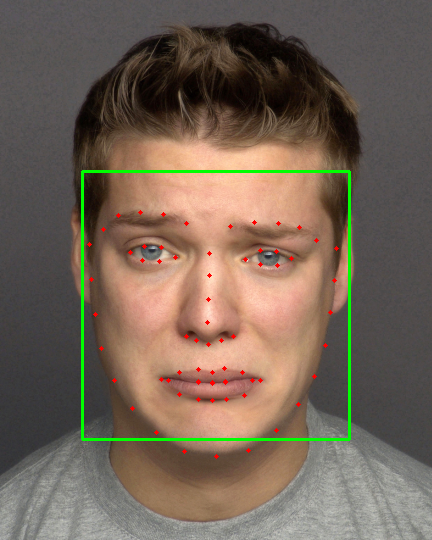
\includegraphics[height=5.5cm]{zdjęcia/detected_landmarks_src.png}
		\subcaption{\label{detected_landmarks_src}}
	\end{subfigure}
	\begin{subfigure}{0.35\textwidth}
		\centering
		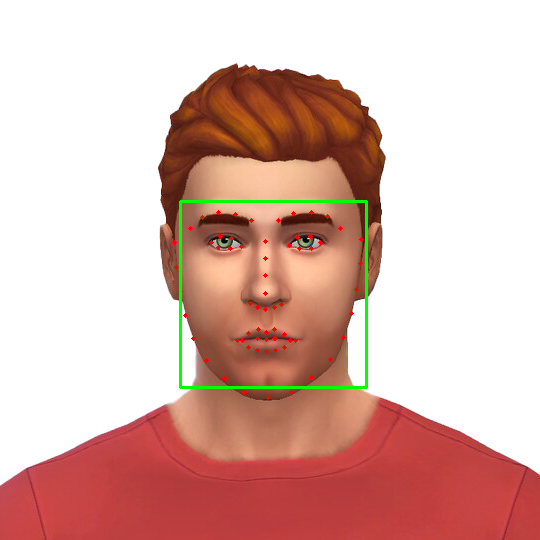
\includegraphics[height=5.5cm]{zdjęcia/detected_landmarks_avatar.png}
		\subcaption{\label{detected_landmarks_avatar}}
	\end{subfigure}
	
	\caption{\label{fig:detectedLandmarks}Twarz i punkty wykryte na obrazie źródłowym \protect\subref{detected_landmarks_src} oraz na awatarze \protect\subref{detected_landmarks_avatar}.}
\end{figure}

Wybrane funkcje zdają się być wystarczające do osiągnięcia zamierzonego rezultatu. Można założyć, iż przetwarzane obrazy zawierają dobrze widoczny obszar twarzy ustawionej w pozycji frontowej. Z tego powodu dokładność działania narzędzia wykrywającego twarz oraz punkty charakterystyczne jest wysoka.


\begin{minted}
[
frame=lines,
label=Wykrycie twarzy oraz punktów charakterystycznych,
framesep=2mm,
baselinestretch=1.2,
breaklines,
bgcolor=white,
fontsize=\footnotesize,
linenos
]
{python}
def detect_face_and_landmarks(img):
    detector = dlib.get_frontal_face_detector()
    predictor = dlib.shape_predictor('./data/shape_predictor_68_face_landmarks.dat')

    gray = cv2.cvtColor(imutils.resize(img), cv2.COLOR_BGR2GRAY)
    rects = detector(gray, 1)
    facial_landmarks = []

    if rects:
        for rect in rects:
            facial_landmarks = predictor(gray, rect)
            facial_landmarks = face_utils.shape_to_np(facial_landmarks)

    return img, facial_landmarks
\end{minted}

Efektem wizualnym użycia powyższej funkcji są obrazy przedstawione na Rys.\ref{fig:detectedLandmarks}. Na każdym ze zdjęć została zlokalizowana twarz, którą zaznaczono zielonym prostokątem oraz jej kluczowe elementy, w postaci 68 punktów oznaczonych kolorem czerwonym. W następnych etapach posłużą one jako baza, na której będą wykonywane wszelkie operacje. 

% \inputminted[firstline=2, lastline=12]{octave}{BitXorMatrix.m}
\section{Triangulacja zbioru punktów}
Kolejnym etapem działania algorytmu animacji awatara jest triangulacja zbioru punktów charakterystycznych, zlokalizowanych na obszarze twarzy obrazu źródłowego. Celem jej zastosowania jest podział przestrzeni na nieskomplikowane trójkąty posiadające ostre kąty, co zapewni przejrzystość i równomierność figur.

W bibliotece OpenCV dostępne są funkcje, generujące triangulację Delone dla zestawu punktów. Ich użycie jest bardzo proste i intuicyjne. Z wykorzystaniem modułu Subdiv2D( Rect rect ), dla którego parametrem wejściowym jest prostokątny obszar obejmujący wszystkie istotne punkty, zostaje wygenerowany pusty obiekt. Następnie za pomocą funkcji insert() można dodać do niego listę elementów charakterystycznych, dla których chcemy dokonać triangulacji. Ostatnim krokiem jest wywołanie funkcji getTriangleList(), która zwraca listę trójkątów wygenerowanych przez algorytm. 

\begin{minted}
[
frame=lines,
label=Triangulacja Delone dla zbioru punktów,
framesep=2mm,
baselinestretch=1.2,
breaklines,
bgcolor=white,
fontsize=\footnotesize,
linenos
]
{python}
def delaunay_triangulation(src_points, avatar_points):
    points_list = list(src_points)
    delaunay_subdivision = cv2.Subdiv2D((*src_points.min(axis=0), *src_points.max(axis=0)))
    delaunay_subdivision.insert(points_list)

    for x1, y1, x2, y2, x3, y3 in delaunay_subdivision.getTriangleList():
        indexes_set = [(src_points == single_point).all(axis=1).nonzero()[0][0]
                       for single_point in [[x1, y1], [x2, y2], [x3, y3]]]

        src_triangles = generate_xy_for_indexes(src_points, indexes_set)
        avatar_triangles = generate_xy_for_indexes(avatar_points, indexes_set)
        yield [np.array(src_triangles), np.array(avatar_triangles)]
        

def generate_xy_for_indexes(points, indexes):
    return [points[single_index] for single_index in indexes]
\end{minted}

Funkcja zaimplementowana w celu rozwiązania tej części problemu generuje opisaną powyżej triangulację. Kolejną istotną kwestią jest wyodrębnienie analogicznych trójkątów z obydwu list punktów. Moduł getTriangleList() zwraca współrzędne wszystkich wierzchołków każdego z wygenerowanych trójkątów. W prosty sposób można odnaleźć ich indeksy w zbiorze punktów charakterystycznych obrazu źródłowego, a następnie zidentyfikować analogiczne elementy w zbiorze punktów wygenerowanych z obrazu awatara.

\begin{figure}[h]
	\centering
	\begin{subfigure}{0.35\textwidth}
		\centering
		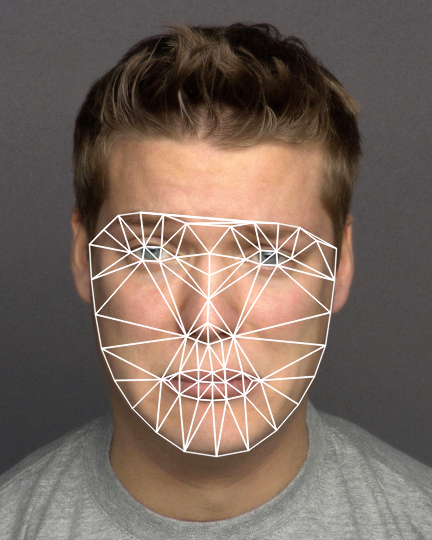
\includegraphics[height=5.5cm]{zdjęcia/triangulation_src.png}
		\subcaption{\label{triangulation_src}}
	\end{subfigure}
	\begin{subfigure}{0.35\textwidth}
		\centering
		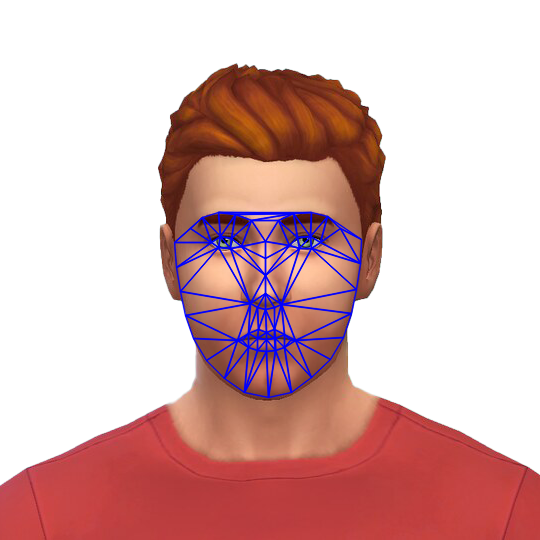
\includegraphics[height=5.5cm]{zdjęcia/triangulation_avatar.png}
		\subcaption{\label{triangulation_avatar}}
	\end{subfigure}
	
	\caption{\label{fig:triangulation}Triangulacja punktów char. obrazu źródłowego \protect\subref{triangulation_src} oraz awatara \protect\subref{triangulation_avatar}.}
\end{figure}

Na Rys. \ref{fig:triangulation} można zaobserwować efekt działania tej części programu. Na pierwszym obrazie zaznaczono trójkąty otrzymane w wyniku zastosowania triangulacji, natomiast na drugim zaznaczono analogiczne trójkąty.




\section{Transformacja trójkątów}
No to tutaj jak to się odbywa, czyli dłuższa sprawa w sumie. Trzeba dać kod, może nie cały plus jakieś zdjęcia, że trójkąty awatara modyfikowane do trójkątów z src, a potem sklejane w maskę. 
tutaj kolejna funkcja, czyli czysta transformacja poprzez te funkcje warp itd itp
\begin{minted}
[
frame=lines,
framesep=2mm,
baselinestretch=1.2,
breaklines,
bgcolor=white,
fontsize=\footnotesize,
linenos
]
{python}
def animate_avatar(avatar_img, avatar_points, src_img, src_points):
    new_avatar_face = np.zeros(src_img.shape, np.uint8)

    for src_triangle_points, avatar_triangle_points in delaunay_triangulation(src_points, avatar_points):
        avatar_img_cropped, avatar_triangle, _ = crop_single_triangle(avatar_triangle_points, avatar_img)
        src_img_cropped, src_triangle, b_rect = crop_single_triangle(src_triangle_points, src_img)

        warped_triangle = transform_triangle(avatar_triangle, avatar_img_cropped, src_triangle, src_img_cropped)
        add_triangle_to_new_face_area(new_avatar_face, warped_triangle, b_rect)

    return generate_new_face(avatar_img, avatar_points, new_avatar_face, src_points)


def crop_single_triangle(single_triangle, img):
    b_rect = cv2.boundingRect(single_triangle)
    triangle_img = [(indexes[0] - b_rect[0], indexes[1] - b_rect[1]) for indexes in single_triangle]
    cropped_img = img[b_rect[1]:b_rect[1] + b_rect[3], b_rect[0]:b_rect[0] + b_rect[2]]

    return cropped_img, triangle_img, b_rect


def transform_triangle(avatar_triangle, avatar_img_cropped, src_triangle, src_img_cropped):
    transform_matrix = cv2.getAffineTransform(np.float32(avatar_triangle), np.float32(src_triangle))

    warped_triangle = cv2.warpAffine(avatar_img_cropped, transform_matrix,
                                     (src_img_cropped.shape[1], src_img_cropped.shape[0]), None,
                                     flags=cv2.INTER_LINEAR, borderMode=cv2.BORDER_REFLECT_101)

    mask = np.zeros(src_img_cropped.shape, dtype=np.uint8)
    mask = cv2.fillConvexPoly(mask, np.int32(src_triangle), (1.0, 1.0, 1.0), 16, 0)
    warped_triangle *= mask

    return warped_triangle


def add_triangle_to_new_face_area(new_face, warped_triangle, b_rect):
    (x, y, w, h) = b_rect
    new_face_gray = cv2.cvtColor(new_face[y: y + h, x: x + w], cv2.COLOR_BGR2GRAY)
    _, mask = cv2.threshold(new_face_gray, 0, 255, cv2.THRESH_BINARY_INV)
    warped_triangle = cv2.bitwise_and(warped_triangle, warped_triangle, mask=mask)

    new_face[y: y + h, x: x + w] += warped_triangle
\end{minted}

\section{Nałożenie maski}

\begin{minted}
[
frame=lines,
framesep=2mm,
baselinestretch=1.2,
breaklines,
bgcolor=white,
fontsize=\footnotesize,
linenos
]
{python}
def generate_new_face(avatar_img, avatar_points, new_avatar_face, src_points):
    transform = PiecewiseAffineTransform()
    transform.estimate(choose_specific_points(avatar_points), choose_specific_points(src_points))

    face = warp(new_avatar_face, transform, output_shape=avatar_img.shape, order=0, mode='wrap')
    face = cv2.normalize(face, None, 0, 255, cv2.NORM_MINMAX, cv2.CV_8U)

    face_gray = cv2.cvtColor(face, cv2.COLOR_BGR2GRAY)
    _, mask = cv2.threshold(face_gray, 0, 255, cv2.THRESH_BINARY_INV)
    new_avatar_img = cv2.bitwise_and(avatar_img, avatar_img, mask=mask)

    new_avatar_img += face

    return new_avatar_img
\end{minted}

No to jak wygląda maska przed rozciągnięciem, a jak po, plus ta funkcja która tam za to odpowiada. W sumie tą funkcję choose można tylko opisać, tutaj pasuje też załączyć zdjęcie z zaznaczonymi 

\begin{figure}[h]
	\centering
	\begin{subfigure}{0.35\textwidth}
		\centering
		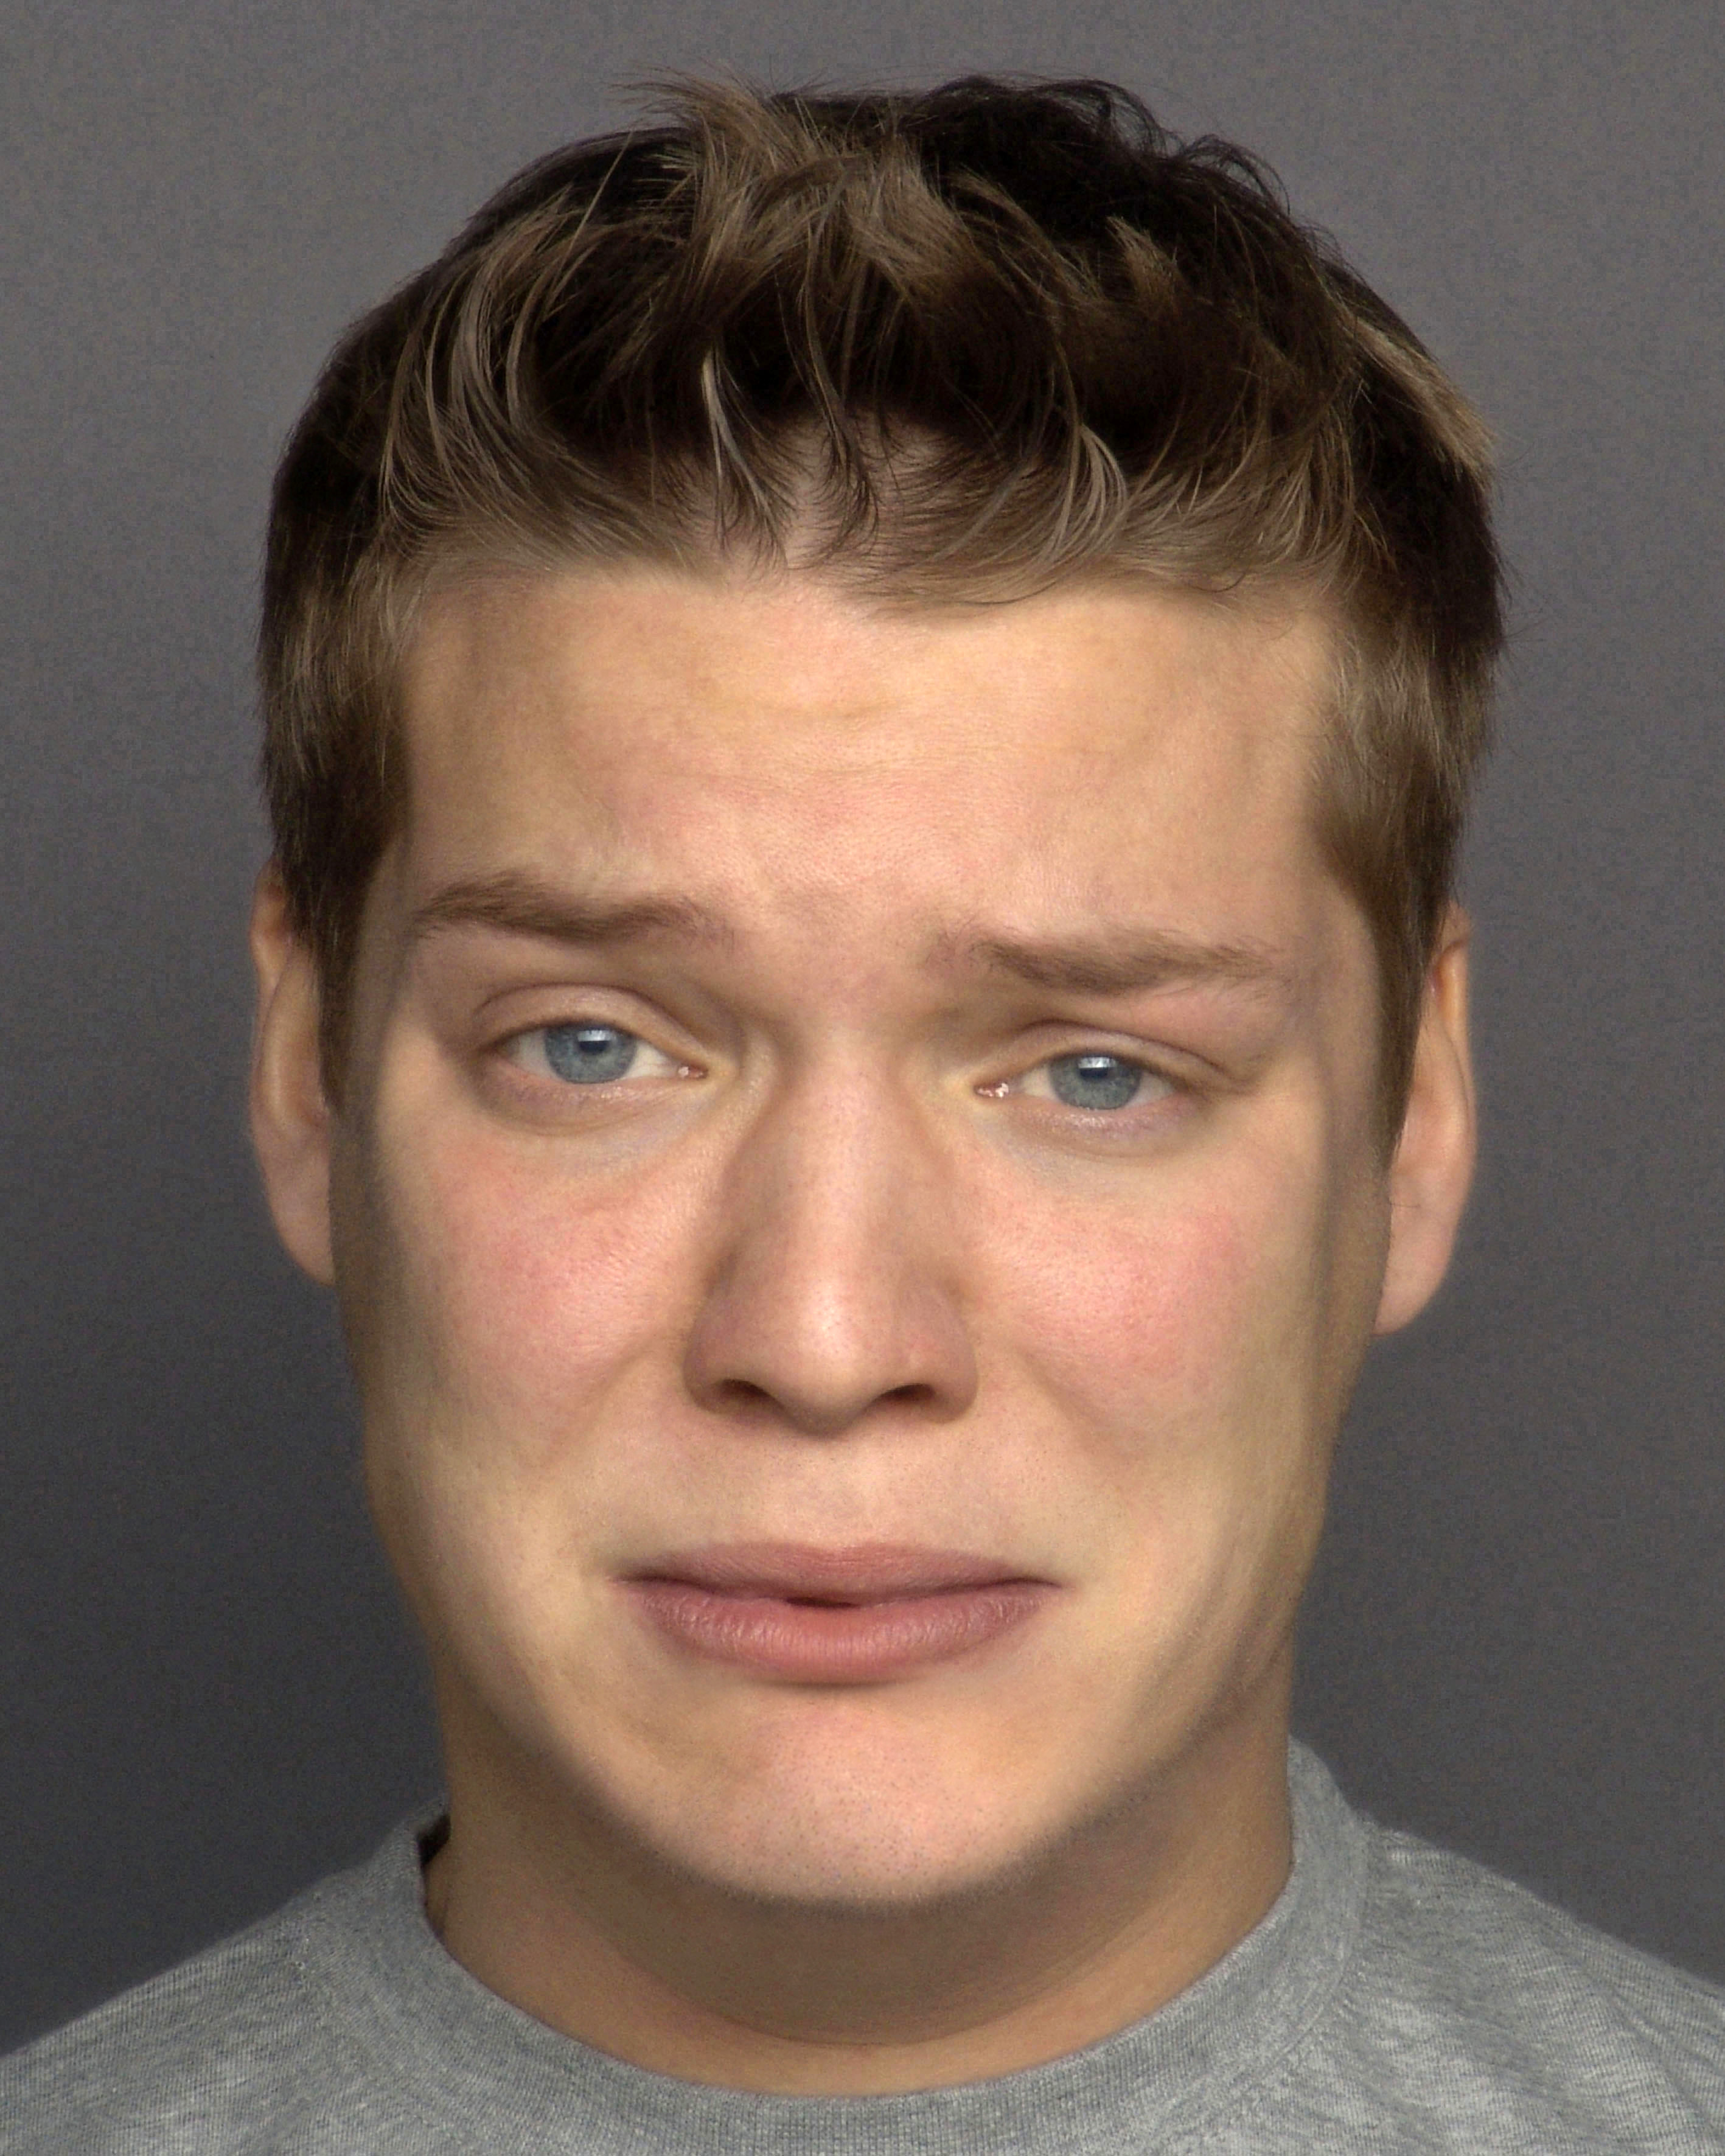
\includegraphics[height=5.5cm]{zdjęcia/src_img.jpg}
		\subcaption{\label{src_img}}
	\end{subfigure}
	\begin{subfigure}{0.35\textwidth}
		\centering
		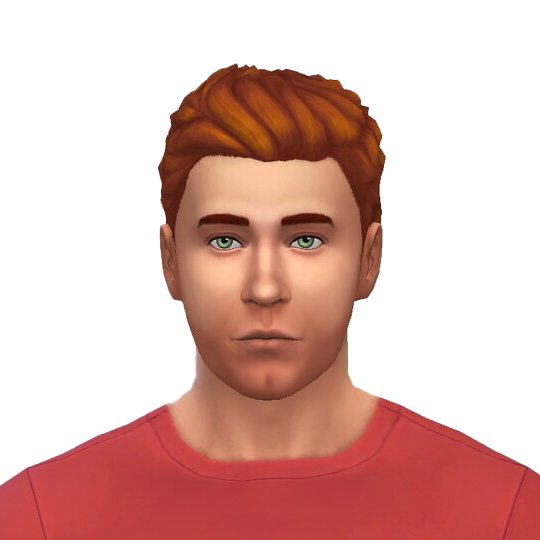
\includegraphics[height=5.5cm]{zdjęcia/avatar.png}
		\subcaption{\label{avatar}}
	\end{subfigure}
	\begin{subfigure}{0.35\textwidth}
		\centering
		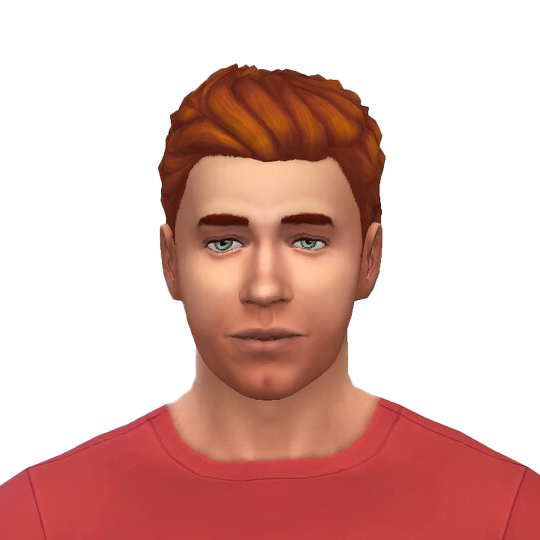
\includegraphics[height=5.5cm]{zdjęcia/result_avatar.png}
		\subcaption{\label{result_avatar}}
	\end{subfigure}
	
	\caption{\label{fig:result}Rezultat działania algorytmu animacji awatara \protect\subref{result_avatar} na zdjęciu źródłowym \protect\subref{src_img} oraz awatarze \protect\subref{avatar}.}
\end{figure}




\chapter{Ewaluacja i rezultaty}
\label{cha:ewaluacjaIRezultaty}
Poniższy rozdział zawiera opis testów przeprowadzonych w celu zbadania poprawności działania algorytmu animacji awatara. Przedstawiono w nim również otrzymane rezultaty i wnioski płynące z opracowanej walidacji.

% %---------------------------------------------------------------------------

\section{Sposób testowania}
Uprzednie przetestowanie stworzonego programu to kluczowa kwestia, dzięki której łatwiej wykryć błędy mogące pojawić się podczas użytkowania danego oprogramowania. Istotna jest również opinia osób testujących program. Niejednokrotnie zwracają oni uwagę na braki, których uzupełnienie potrafi zdecydowanie usprawnić korzystanie z aplikacji.

\begin{figure}[h]
	\centering
	\begin{subfigure}{0.35\textwidth}
		\centering
		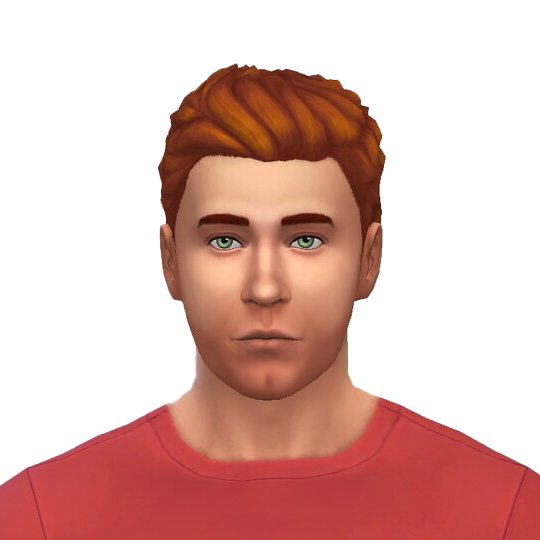
\includegraphics[height=4cm]{zdjęcia/1.png}
		\subcaption{\label{avatar_1}}
	\end{subfigure}
	\begin{subfigure}{0.35\textwidth}
		\centering
		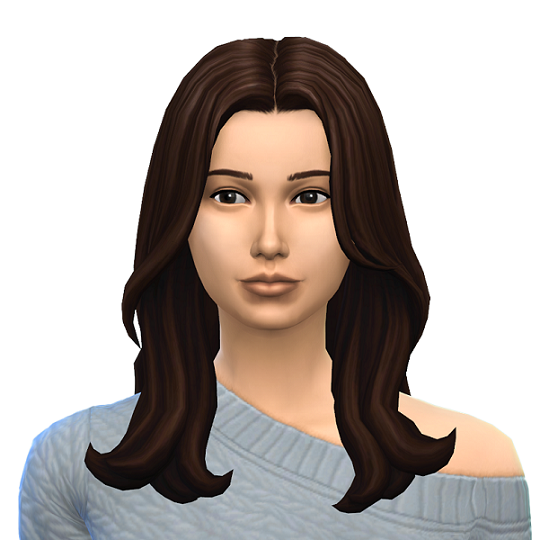
\includegraphics[height=4cm]{zdjęcia/2.png}
		\subcaption{\label{avatar_2}}
	\end{subfigure}
	\begin{subfigure}{0.35\textwidth}
		\centering
		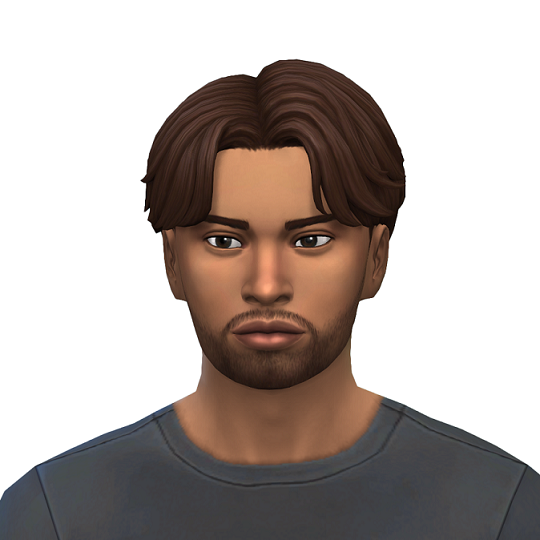
\includegraphics[height=4cm]{zdjęcia/3.png}
		\subcaption{\label{avatar_3}}
	\end{subfigure}
	\begin{subfigure}{0.35\textwidth}
		\centering
		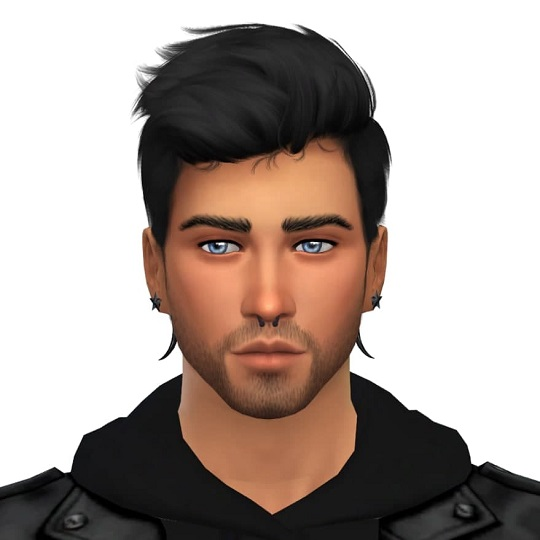
\includegraphics[height=4cm]{zdjęcia/4.png}
		\subcaption{\label{avatar_4}}
	\end{subfigure}
	
	\caption{\label{fig:avatars}Awatary użyte do przetestowania algorytmu}
\end{figure}

W czasie tworzenia algorytmu animacji awatara zostały przeprowadzone testy manualne poszczególnych funkcji, co pomogło usprawnić niektóre moduły i dopracować logikę ich działania. Ze względu na prostotę programu, stworzonego na potrzeby tej pracy inżynierkiej, wykonywanie bardziej zaawansowanych testów samego oprogramowania nie było konieczne.

Ważnym elementem stało się przetestowanie efektywności działania algorytmu na zarejestrowanych obrazach lub gotowych zbiorach danych, co wcześniej zostało określone w założeniach projektowych (sekcja \ref{sec:zalozeniaProjektu}). Z tego powodu przeprowadzono testy użyteczności, które zostały podzielone na dwie części. W każdej z nich modyfikowano zdjęcia czterech różnych awatarów (Rys. \ref{fig:avatars}), co pozwoliło na dokładniejsze przetestowanie algorytmu.

Dobór zdjęć użytych do badań nie był przypadkowy. W ramach niniejszej pracy jako awatar rozumie się nierealną cyfrową postać mającą formę osobową. Ważną cechą jest prostota takiego charakteru - wyraźne rysy twarzy, brak cieni. Ze względu na owe wymagania do testów wybrano podobizny z popularnej gry symulacyjnej The Sims 4, które zostały udostępnione na forum~\cite{avatars}.

% %---------------------------------------------------------------------------

\section{Walidacja z użyciem aplikacji}
Pierwsza część przeprowadzonych testów obejmuje wykorzystanie aplikacji webowej w celu zbadania efektywności działania algorytmu w przypadku animacji na podstawie obrazu przechwyconego z kamery. 

Na potrzeby przeprowadzonego badania stworzono ankietę składającą się z czterech sekcji, gdzie każda dotyczy modyfikacji innego awatara. Głównym zadaniem ma być ocena rezultatów odwzorowania czterech podstawowych emocji \cite{emotions}, na które składają się:

\begin{itemize}
    \item szczęście,
    \item smutek,
    \item strach/zaskoczenie,
    \item gniew/obrzydzenie.
\end{itemize}

Każda sekcja złożona jest z pięciu pytań:
\begin{itemize}
    \item cztery z nich dotyczą testowania zakładki \textit{Real-time animation}, gdzie awatar jest animowany na podstawie obrazu przechwyconego z kamery,
    \item jedno ma na celu porówananie efektów otrzymanych przez animację opartą na analizowaniu obrazu z kamery z modyfikacją na podstawie wczytanego zdjęcia (zakładka \textit{Select image}).
\end{itemize}

Treść czterech pierwszych pytań, pod którymi kryją się kolejne zadania, różni się między sobą tylko aktualnie testowaną emocją. Dla przykładu pierwsze pytanie ma postać:
\begin{center}
    Odwzorowanie pierwszej podstawowej emocji (szczęście).
\end{center}

W tej części zastosowano ocenianie za pomocą skali od 1 do 5, gdzie konkretnym wartościom odpowiadają następujące etykiety:
\begin{enumerate}
    \item Bardzo słaby
    \item Słaby
    \item Przeciętny
    \item Dobry
    \item Bardzo dobry

\end{enumerate}

\begin{table}[h]
\centering
\begin{tabular}{|c|l|c|c|c|c|c|} 
\hline
\multirow{2}{*}{\textbf{awatar}} & \multicolumn{1}{c|}{\multirow{2}{*}{\textbf{emocja}}} & \multicolumn{5}{c|}{\textbf{ocena}}                                                                                                   \\ 
\cline{3-7}
                                 & \multicolumn{1}{c|}{}                                 & \textbf{1} & \textbf{2} & \textbf{3}                       & \textbf{4}                         & \textbf{5}                          \\ 
\hhline{|=======|}
\multirow{4}{*}{\ref{avatar_1}}        & szczęście                                             & ~ 0\%~~    & ~ 9\%~~    & ~ 0\%~                           & \textcolor[rgb]{0,0.588,0}{~ 45\%} & \textcolor[rgb]{0,0.588,0}{~ 45\%}  \\ 
\cline{2-7}
                                 & smutek                                                & 0\%        & 0\%        & 0\%                              & \textcolor[rgb]{0,0.588,0}{64\%}   & 36\%                                \\ 
\cline{2-7}
                                 & zaskoczenie/strach                                    & 0\%        & 0\%        & 18\%                             & \textcolor[rgb]{0,0.588,0}{45\%}   & 36\%                                \\ 
\cline{2-7}
                                 & gniew/obrzydzenie                                     & 0\%        & 9\%        & 18\%                             & \textcolor[rgb]{0,0.588,0}{36\%}   & \textcolor[rgb]{0,0.588,0}{36\%}    \\ 
\hhline{|=======|}
\multirow{4}{*}{\ref{avatar_2}}           & szczęście                                             & 0\%        & 9\%        & 9\%                              & \textcolor[rgb]{0,0.588,0}{45\%}   & 36\%                                \\ 
\cline{2-7}
                                 & smutek                                                & 0\%        & 27\%       & 9\%                              & \textcolor[rgb]{0,0.588,0}{45\%}   & 18\%                                \\ 
\cline{2-7}
                                 & zaskoczenie/strach                                    & 9\%        & 0\%        & 27\%                             & \textcolor[rgb]{0,0.588,0}{55\%}   & 9\%                                 \\ 
\cline{2-7}
                                 & gniew/obrzydzenie                                     & 9\%        & 18\%       & \textcolor[rgb]{0,0.588,0}{45\%} & 27\%                               & 0\%                                 \\ 
\hhline{|=======|}
\multirow{4}{*}{\ref{avatar_3}}          & szczęście                                             & 0\%        & 0\%        & 9\%                              & \textcolor[rgb]{0,0.588,0}{45\%}   & \textcolor[rgb]{0,0.588,0}{45\%}    \\ 
\cline{2-7}
                                 & smutek                                                & 0\%        & 0\%        & 27\%                             & \textcolor[rgb]{0,0.588,0}{55\%}   & 18\%                                \\ 
\cline{2-7}
                                 & zaskoczenie/strach                                    & 0\%        & 9\%        & 18\%                             & \textcolor[rgb]{0,0.588,0}{36\%}   & \textcolor[rgb]{0,0.588,0}{36\%}    \\ 
\cline{2-7}
                                 & gniew/obrzydzenie                                     & 0\%        & 18\%       & 18\%                             & \textcolor[rgb]{0,0.588,0}{36\%}   & 27\%                                \\ 
\hhline{|=======|}
\multirow{4}{*}{\ref{avatar_4}}         & szczęście                                             & 0\%        & 0\%        & 0\%                              & 18\%                               & \textcolor[rgb]{0,0.588,0}{82\%}    \\ 
\cline{2-7}
                                 & smutek                                                & 0\%        & 9\%        & 0\%                              & \textcolor[rgb]{0,0.588,0}{55\%}   & 36\%                                \\ 
\cline{2-7}
                                 & zaskoczenie/strach                                    & 0\%        & 9\%        & 9\%                              & \textcolor[rgb]{0,0.588,0}{55\%}   & 27\%                                \\ 
\cline{2-7}
                                 & gniew/obrzydzenie                                     & 0\%        & 9\%        & 9\%                              & \textcolor[rgb]{0,0.588,0}{64\%}   & 18\%                                \\
\hline
\end{tabular}
\caption{Wyniki walidacji przeprowadzonej z użyciem aplikacji webowej}
\label{tab:first_test}
\end{table}

Ostatnie, piąte pytanie dotyczy oceny rezultatu osiągniętego w zakładce \textit{Select image} dla danego awatara. Osoba ankietowana powinna wybrać jedno zdjęcie z udostępnionej bazy odwzorowujące emocje, dla której rezultat animacji wypadł najgorzej. Następnie należy ocenić osiągnięty efekt, w stosunku do tego otrzymanego w zakładce \textit{Real-time animation}. Tym razem użyto skali od 1 do 7 gdzie 1 oznacza \textit{zdecydowanie gorszy} efekt, natomiast 7 \textit{zdecydowanie lepszy} wynik.

Przed przystąpieniem do testowania użytkownicy zostali zapoznani z krótką instrukcją, w której zwrócono uwagę na czynniki mogące mieć wpływ na działanie algorytmu:

\begin{enumerate}
    \item Ustaw twarz w pozycji frontowej, tak aby była ona dobrze widoczna w kamerze.
    \item Odsłoń włosy oraz zdejmij okulary.
    \item Staraj się nie wykonywać gwałtownych ruchów w momencie naciskania przycisku \textit{Animate}.
    \item W trakcie oceny rezultatów kieruj się głównie tym, czy emocja została poprawnie odwzorowana.
    \item Możesz wielokrotnie dokonywać animacji dla danej emocji i ocenić sumaryczne rezultaty.
\end{enumerate}

W ankiecie wzięło udział 11 osób w przedziale wiekowym od 19 do 60 lat. Większość z nich korzysta na co dzień z komputera, jednak tylko w podstawowych celach. W trakcie przeprowadzania ankiety nie wyniknęły żadne problemy. Aplikacja działała płynnie, przez co każdej ankietowanej osobie udało się ukończyć zadania bez przeszkód.

Procentowe wyniki ankiety przedstawiono w powyższej tabeli~(Tab.~\ref{tab:first_test}). Zawarto w niej podsumowane odpowiedzi na pytania 1-4, czyli te dotyczące odwzorowania danej emocji. Dla każdego awatara i poszczególnych emocji dominujące wartości oznaczono kolorem zielonym. 

Analizując wyniki można dojść do następujących wniosków:
\begin{itemize}
    \item najlepsze oceny zanotowano dla awatara \ref{avatar_4}. Odwzorowanie każdej z emocji zostało ocenione jako \textit{dobre} lub \textit{bardzo dobre} średnio w 89\% przypadków,
    \item ocena \textit{bardzo słaby} pojawiła się dwukrotnie, wyłącznie dla awatara \ref{avatar_2},
    \item największa liczba ocen \textit{słaby} oraz \textit{bardzo słaby} wystąpiła dla awatara \ref{avatar_2} (średnio 18\% odpowiedzi).
\end{itemize}

Podsumowując odpowiedzi na ostatnie pytanie, dotyczące porównania efektów osiągniętych w zakładce \textit{Select image} oraz \textit{Real-time animation}, można dojść do poniższych~{spostrzeżeń}:
\begin{itemize}
    \item dla awatara \ref{avatar_1} w 91\% przypadków odpowiedzi skupiają się w przedziale od 4 do 7, co oznacza tendencję w kierunku oceny \textit{zdecydowanie lepszy},
    \item oceny awatara \ref{avatar_2} kumulują się między 1 a 4, co oznacza osiągnięcie głównie gorszych rezultatów,
    \item dla awatara \ref{avatar_3} koncentracja odpowiedzi przypada na przedział 4-7, aż w 45\% zdecydowano że efekt modyfikacji poprzez zakładkę \textit{Select image} jest \textit{zdecydowanie lepszy},
    \item efekty dla ostatniego awatara (\ref{avatar_4}) zostały ocenione bardzo różnorodnie, żadna z odpowiedzi nie wydaje się znacząco dominować.
\end{itemize}


% %---------------------------------------------------------------------------

\section{Walidacja na zbiorze danych}
Drugi etap testów dotyczy oceny rezultatów algorytmu osiągniętych z wykorzystaniem gotowego zbioru danych. Celem tej części jest ocena wcześniej zmodyfikowanych awatarów. Powinna ona zapewnić przejrzyste, nieobarczone błędem wnioski. Wyniki walidacji przedstawionej we wcześniejszej sekcji są narażone na przekłamanie, ponieważ efekty zależą od mimiki poszczególnych osób biorących udział w badaniu.

Przygotowanie danych przebiegało w następujący sposób:
\begin{itemize}
    \item wykorzystano bazę zdjęć zawierającą podobizny mężczyzn oraz kobiet z różnymi wyrazami twarzy, odpowiadającymi określonym emocjom,
    \item dla każdej emocji, których podstawowy podział został podany w powyższym rozdziale, wybrano po jednym zdjęciu,
    \item na podstawie określonych obrazów dokonano modyfikacji każdego awatara. Finalnie otrzymano 16 przekształconych podobizn.
\end{itemize}

\begin{table}[h]
\centering
\begin{tabular}{|c|c|c|c|c|} 
\hline & \multicolumn{4}{c|}{\textbf{awatar}} \\ 
\hline
\textbf{emocja} & \textbf{\ref{avatar_1}} & \textbf{\ref{avatar_2}} & \textbf{\ref{avatar_3}} & \textbf{\ref{avatar_4}} \\ 
\hline
szczęście & 74\% & 70\% & 85\% & \textcolor[rgb]{0,0.502,0}{\textbf{100\%}} \\ 
\hline
smutek & 78\% & \textcolor[rgb]{0,0.502,0}{~\textbf{93\%}} & 85\% & 85\% \\ 
\hline
zaskoczenie/strach & \textcolor[rgb]{0,0.502,0}{~\textbf{93\% }} & 74\% & 63\% & 63\% \\ 
\hline
gniew/obrzydzenie & 78\% & 41\% & \textcolor[rgb]{0,0.502,0}{~\textbf{96\%}} & 67\% \\ 
\hline
\bottomrule
\begin{tabular}[c]{@{}c@{}}sumaryczna poprawność\end{tabular} & 81\% & {\cellcolor{red}}\textcolor{white}{69\%}  & {\cellcolor[rgb]{0,0.502,0}}\textcolor{white}{82\%} & 79\% \\
\hline
\end{tabular}
\caption{Ocena rezultatów osiągniętych z użyciem gotowego zbioru danych}
\label{tab:second_test}
\end{table}

\newpage
Ankieta utworzona na potrzeby badania składa się z  16 pytań, każde z nich posiada cztery możliwe odpowiedzi:

\begin{enumerate}
    \item szczęście,
    \item smutek,
    \item strach/zaskoczenie,
    \item gniew/obrzydzenie.
\end{enumerate}

Zadaniem osoby ankietowanej była próba dopasowania emocji, którą odzwierciedla zmodyfikowany wyraz twarzy awatara. W celu łatwiejszego uporządkowania wyników zastosowano punktację 0-1. 

W ankiecie wzięło udział 27 osób w różnym przedziale wiekowym. Poniżej przedstawiono wartości najważniejszych parametrów otrzymanych wyników:
\begin{itemize}
    \item maksymalna liczba zdobytych punktów - 16
    \item najniższy wynik - 9
    \item średni wynik - 12,44/16
    \item mediana - 12
\end{itemize}

\begin{figure}[h]
	\centering
	\begin{subfigure}{0.35\textwidth}
		\centering
		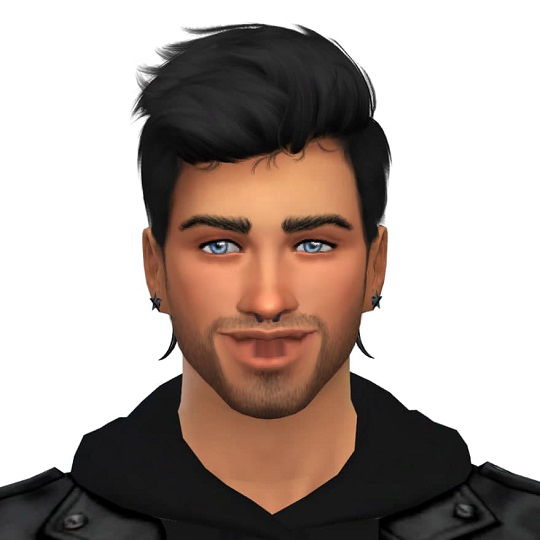
\includegraphics[height=4.5cm]{zdjęcia/av-4_happiness_2.png}
		\subcaption{\label{av-4_happiness_2}}
	\end{subfigure}
	\begin{subfigure}{0.35\textwidth}
		\centering
		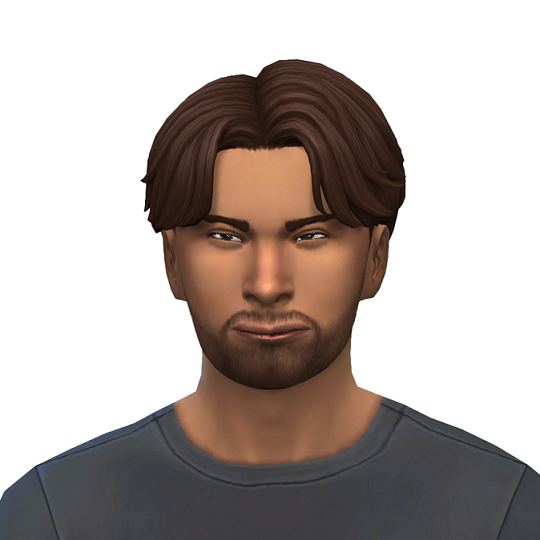
\includegraphics[height=4.5cm]{zdjęcia/av-3_anger_2.png}
		\subcaption{\label{av-3_anger_2}}
	\end{subfigure}

	
	\caption{\label{fig:best_results}Najtrafniej odgadnięte odwzorowania}
\end{figure}

Wyniki procentowe otrzymane po przeprowadzeniu badania zawarto w tabeli \ref{tab:second_test}. Po szczegółowej analizie, można zauważyć, że:
\begin{itemize}
    \item najwyżej oceniono awatar \ref{avatar_3} (82\% poprawnych odpowiedzi), a najgorzej \ref{avatar_2} (poprawność na poziomie 69\%),
    \item w odwzorowaniu szczęścia najwyższy wynik, bo aż 100\% zanotowano dla awatara \ref{avatar_4},
    \item smutny wyraz twarzy najtrafniej przyporządkowywano dla awatara \ref{avatar_2} (93\%),
    \item w przypadku emocji zaskoczenia/strachu najwyższą poprawność dopasowania otrzymano dla awatara \ref{avatar_1} (93\%),
    \item najlepszy rezultat dla gniewu/obrzydzenia osiągnięto na awatarze \ref{avatar_3} (96\%).
\end{itemize}

Obrazy, których odzwierciedlane emocje przyporządkowano z najlepszą skutecznością (kolejno 100\% oraz 96\%) przedstawiono na Rys. \ref{fig:best_results}. Według ankietowanych obraz \ref{av-4_happiness_2} bardzo dobrze oddaje szczęście, mimo pewnego defektu w postaci braku uzębienia. Natomiast Rys.~\ref{av-3_anger_2} poprawnie ukazuje gniew/obrzydzenie poprzez odpowiednie ułożenie ust oraz oczu. 

% %---------------------------------------------------------------------------

\section{Wnioski}
Przeprowadzone testy pomogły sprawdzić poprawność algorytmu zaimplementowanego w niniejszej pracy dyplomowej. Według użytkowników algorytm zapewnia dobre efekty, a stworzona aplikacja jest przyjemna i intuicyjna w użyciu. Wiele osób stwierdziło, iż udział w badaniu był przyjemny i przysporzył sporo rozrywki.

Badania opisane w powyższym rozdziale pozwoliły na wykrycie wad oraz zdefiniowanie potencjalnych kierunków rozwoju i usprawnienia algorytmu. Kilku użytkowników zwróciło uwagę na brak uzębienia animowanych awatarów, który rozpraszał w trakcie testowania programu. Pojedyncza osoba wspomniała także o braku uwzględniania ułożenia brwi. Niewykluczone, że poprawa tego elementu zdecydowanie udoskonaliłaby odwzorowanie emocji.

Głównym celem było zbadanie jakości działania programu względem doboru awatara. Okazało się, że efektywność algorytmu w dużym stopniu zależy od obrazu, na którym następuje animacja. W pierwszej części testów najwyżej oceniono obraz \ref{avatar_4}, a w drugiej \ref{avatar_3}. Natomiast w obu najniżej oceniono awatar \ref{avatar_2}, na którym podczas modyfikacji pojawiało się sporo artefaktów psujących efekt animacji. Jak widać, dla różnych awatarów otrzymano odmienne wyniki. W przypadku kobiety znajdującej się na obrazie \ref{avatar_2} włosy nachodzące na twarz mogły negatywnie wpłynąć na rezultaty.

Istotną kwestią była także część, w której porównywano działanie algorytmu na gotowych obrazach z animacją \textit{real-time}. Dla awatarów ocenionych najwyżej efekty z obydwu zakładek były porównywalne, jednak dla awatara ocenionego najgorzej efektywność animacji na podstawie gotowych obrazów dawała lepsze wyniki. Wynika z tego, iż poprawnie użyta zakładka \textit{real-time} nie wpływała negatywnie na wizualicję, ale może poprawić jej efekt w przypadku animacji na niekorzystnym awatarze. Warto pamiętać, że rezultaty są mocno zależne od mimiki danej osoby, dla każdej z nich inny awatar sprawdzał się lepiej. 

Uważam, iż przeprowadzone testy przebiegły pomyślnie. Stworzona aplikacja okazała się dobrym narzędziem walidacji. Ewaluacja na gotowym zbiorze danych pomogła potwierdzić otrzymane wyniki oraz zwrócić uwagę na dodatkowe ścieżki rozwoju.




\chapter{Podsumowanie}
\label{cha:podsumowanie}
Głównym celem niniejszego projektu dyplomowego było opracowanie algorytmu animacji awatara. Zaimplementowana metoda miała opierać swoje działanie na identyfikacji punktów charakterystycznych twarzy, będących podstawą dalszych transformacji. W ramach walidacji oprogramowania należało napisać nieskomplikowaną aplikację webową.

Stworzenie owego algorytmu okazało się czasochłonne i wymagało wielu modyfikacji oraz zmian koncepcji, jednak zakończyło się sukcesem.  Utworzony program zdaje się działać poprawnie i pozwala osiągnąć całkiem dobre efekty. Oczywiste jest, że aktualna wersja programu nie jest idealna i z pewnością można ją dopracować, ale spełnia określone na początku wymagania. Udało się także zbudować aplikację webową, która ułatwiła przedstawienie algorytmu oraz jego przetestowanie. 

% %---------------------------------------------------------------------------

\section{Weryfikacja początkowych założeń}
W pierwszym rozdziale owej pracy (sekcja \ref{sec:zalozeniaProjektu}) wymieniono założenia, które w etapie końcowym powinien spełniać stworzony projekt. Poniżej zostanie przedstawiona ich analiza oraz weryfikacja osiągniętych efektów:

\begin{itemize}
    \item Działanie algorytmu miało zostać powiązane z analizą punktów charakterystycznych twarzy, co w stu procentach osiągnięto. Algorytm rozpoczyna działanie od ich wykrycia. Na tej podstawie odbywają się kolejne etapy, które dotyczą modyfikacji obszarów wyznaczonych przez dane punkty.
    \item Samą identyfikację punktów udało się zrealizować z wykorzystaniem biblioteki dlib, dzięki której odbywa się wykrycie twarzy oraz jej istotnych elementów. 
    \item Po stworzeniu projektu algorytm przetestowano według planu, na gotowym zbiorze danych, co umożliwiło sprawdzenie poprawności jego działania.
    \item Zgodnie z planem, zaimplementowano prostą aplikację webową, wykorzystaną do walidacji algorytmu. Moim osobistym założeniem było utworzenie filtra animującego awatar w czasie rzeczywistym. Niestety z powodu długiego czasu działania funkcji \textit{warp()} z biblioteki scikit-image, nie udało się go zrealizować. Nie ukrywam, że bardzo zależy mi, aby w przyszłości wdrożyć ten element.
\end{itemize}

Podsumowując, wszystkie założenia postawione na początku tworzenia programu zostały zrealizowane. Dzięki cennym informacjom zdobytym podczas przeprowadzonych badań pozostaje kwestia jego optymalizacji i dalszego rozwoju.

% %---------------------------------------------------------------------------

\section{Możliwy rozwój projektu}
Działanie algorytmu zaimplementowanego w trakcie tworzenia niniejszej pracy dyplomowej można usprawnić na wiele sposobów. Udoskonalenie niektórych etapów z pewnością poprawiłoby osiągane rezultaty. Pierwszym ważnym elementem jest próba dodania rozwiązania, które zapewni lepszy efekt wizualny w przypadku, gdy usta awatara się rozszerzają - warto zastanowić się nad kwestią pokazania uzębienia.

Ponadto dotychczasowy czas działania niektórych funkcji wykorzystanych w programie zdaje się być zbyt długi. Niewykluczone, że lepszym rozwiązaniem byłoby zastąpienie ich wydajniejszymi modułami - być może należy takowe opracować. Prawdopodobnie poprawa czasu działania algorytmu możliwiłaby udoskonalenie aplikacji - stworzenie filtra animującego awatar w czasie rzeczywistym.

Uważam również, że warto przemyśleć etap nałożenia maski i być może spróbować rozwiązać go w inny sposób. W tym momencie maska dopasowywana jest poprzez wykorzystanie funkcji z biblioteki scikit-image, która transformuje obraz na podstawie wybranych punktów charakterystycznych. Rezultat wydawał się zadowalający, jednakże podczas testów dwie osoby zwróciły uwagę na brak animacji brwi, co w tym momencie nie jest możliwe, ze względu na to że owe punkty biorą udział w transformacji - ich modyfikacja jest niemożliwa.

Niewykluczone, że dobranie modelu z inną ilością punktów charakterystycznych również wpłynęłoby na poprawę efektów jakie zapewnia działanie algorytmu.

Wydaje mi się, że wszystkie wymienione wyżej propozycje poprawiłyby efekty, które w tym momencie można osiągnąć używając algorytmu animacji awatara. Warto również rozwinąć aplikację stworzoną na potrzeby ewaluacji, dokładniej przetestować jej działanie i popracować nad interfejsem graficznym.
% \chapter{Opis używanych pojęć}
% \label{}
% \begin{itemize}
%     \item punkty charakterystyczne (ang. landmarks) - punkty rozpoznawcze twarzy wykrywane na obrazie. W kontekście tejże pracy, używane w celu lokalizacji i reprezentacji najistotniejszych obszarów ludzkiej twarzy. Mowa tutaj o linii szczęki, ust, nosa, oczu i brwi.
%     \item awatar - tożsamość internetowa, czyli cyfrowa postać odzwierciedlająca wizerunek danej osoby. Awatary używane są w grach komputerowych, na forach i w mediach społecznościowych. Zazwyczaj przybierają dowolną formę (człowiek, zwierzę). W ramach niniejszej pracy jako awatar rozumie się nierealną cyfrową postać mającą formę osobową. Ważną kwestią jest prostota takiego charakteru - wyraźne rysy twarzy, brak cieni.
%     \item predictor - w kontekscie wykrywania twarzy, model glebokiego uczenia
%     \item detector - to samo, co to jest w kontekscie tego algorytmu
%     \item triangulacja - metoda podzialu figury geometrycznej itd itp
%     \item sympleksy
%     \item maska - tutaj kwestia zapytania, trzeba ogarnac poprawna definicje i sprawdzic czy dobrze jej uzywam
% \end{itemize}



% itd.
% \appendix
% \include{dodatekA}
% \include{dodatekB}
% itd.

\printbibliography
\end{document}
